% Options for packages loaded elsewhere
\PassOptionsToPackage{unicode}{hyperref}
\PassOptionsToPackage{hyphens}{url}
%
\documentclass[
]{book}
\usepackage{amsmath,amssymb}
\usepackage{lmodern}
\usepackage{ifxetex,ifluatex}
\ifnum 0\ifxetex 1\fi\ifluatex 1\fi=0 % if pdftex
  \usepackage[T1]{fontenc}
  \usepackage[utf8]{inputenc}
  \usepackage{textcomp} % provide euro and other symbols
\else % if luatex or xetex
  \usepackage{unicode-math}
  \defaultfontfeatures{Scale=MatchLowercase}
  \defaultfontfeatures[\rmfamily]{Ligatures=TeX,Scale=1}
\fi
% Use upquote if available, for straight quotes in verbatim environments
\IfFileExists{upquote.sty}{\usepackage{upquote}}{}
\IfFileExists{microtype.sty}{% use microtype if available
  \usepackage[]{microtype}
  \UseMicrotypeSet[protrusion]{basicmath} % disable protrusion for tt fonts
}{}
\makeatletter
\@ifundefined{KOMAClassName}{% if non-KOMA class
  \IfFileExists{parskip.sty}{%
    \usepackage{parskip}
  }{% else
    \setlength{\parindent}{0pt}
    \setlength{\parskip}{6pt plus 2pt minus 1pt}}
}{% if KOMA class
  \KOMAoptions{parskip=half}}
\makeatother
\usepackage{xcolor}
\IfFileExists{xurl.sty}{\usepackage{xurl}}{} % add URL line breaks if available
\IfFileExists{bookmark.sty}{\usepackage{bookmark}}{\usepackage{hyperref}}
\hypersetup{
  pdftitle={IoTeX Documentation Review},
  pdfauthor={Ricky Esclapon},
  hidelinks,
  pdfcreator={LaTeX via pandoc}}
\urlstyle{same} % disable monospaced font for URLs
\usepackage{graphicx}
\makeatletter
\def\maxwidth{\ifdim\Gin@nat@width>\linewidth\linewidth\else\Gin@nat@width\fi}
\def\maxheight{\ifdim\Gin@nat@height>\textheight\textheight\else\Gin@nat@height\fi}
\makeatother
% Scale images if necessary, so that they will not overflow the page
% margins by default, and it is still possible to overwrite the defaults
% using explicit options in \includegraphics[width, height, ...]{}
\setkeys{Gin}{width=\maxwidth,height=\maxheight,keepaspectratio}
% Set default figure placement to htbp
\makeatletter
\def\fps@figure{htbp}
\makeatother
\setlength{\emergencystretch}{3em} % prevent overfull lines
\providecommand{\tightlist}{%
  \setlength{\itemsep}{0pt}\setlength{\parskip}{0pt}}
\setcounter{secnumdepth}{-\maxdimen} % remove section numbering
\ifluatex
  \usepackage{selnolig}  % disable illegal ligatures
\fi

\title{IoTeX Documentation Review}
\author{Ricky Esclapon}
\date{2021-05-29}

\begin{document}
\frontmatter
\maketitle

\mainmatter
\hypertarget{introduction}{%
\chapter{Introduction}\label{introduction}}

My name is Ricky (ETH-0x8115AfD8DFfCE5579381AD27524b6Feeae917BEF) and
this is my review of the IoTeX documentation for the following bounty on
Gitcoin:
\url{https://gitcoin.co/issue/iotexproject/halogrants/32/100025753}

This document outlines each section from the IoTeX docs with my
comments, \protect\hyperlink{the-internet-of-trusted-things}{starting
with \textbf{Software Tools} page in the next section}.

\hypertarget{software-tools---get-started}{%
\chapter{Software Tools - Get
Started}\label{software-tools---get-started}}

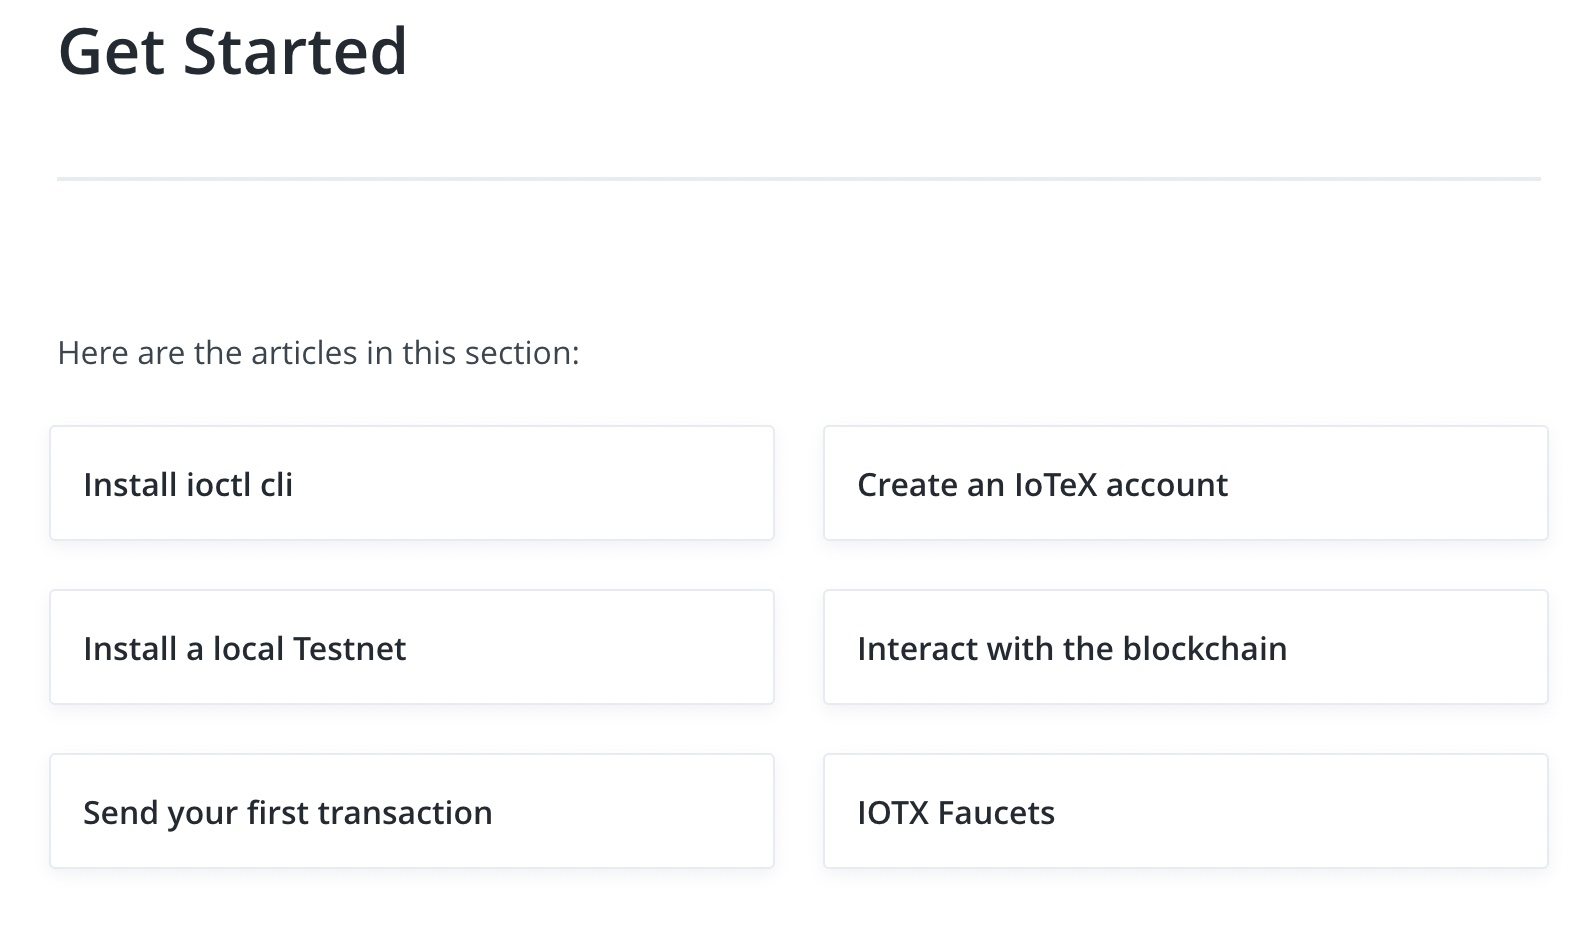
\includegraphics{images/get_started.jpg}

This section is nicely linked, but I think a more narrative approach
would be more effective. I think the links are great and useful for a
user that already has a clear idea of what they want to do and why, but
I think the quick Get Started example should hold the users' hand even
more than this the whole way, and clearly outline why each step will be
necessary.

So I think a good approach here would be to build something specific and
straightforward and walk the user very clearly through the entire
process to keep things more grounded and concrete. From there, I think
it would be better to clearly explain why one needs to install the
\textbf{ioctl cli}, then \textbf{create an account}, then
\textbf{install a local testnet}, then \textbf{interact with the
blockchain}, etc\ldots{} Each step is necessary and serves a specific
purpose, so it would be good to create a quick overview with a sentence
or two detailing why each is necessary before the user actually gets
started. I think it could help add clarity to the actual order of
operations to have a quick explainer as well as a concrete easy project
that users can ground themselves on as they work through the Get Started
quickstart example.

\hypertarget{install-ioctl-cli}{%
\section{Install ioctl cli}\label{install-ioctl-cli}}

Some important notes on this one:
\url{https://docs.iotex.io/software-tools/get-started/install-ioctl-cli}

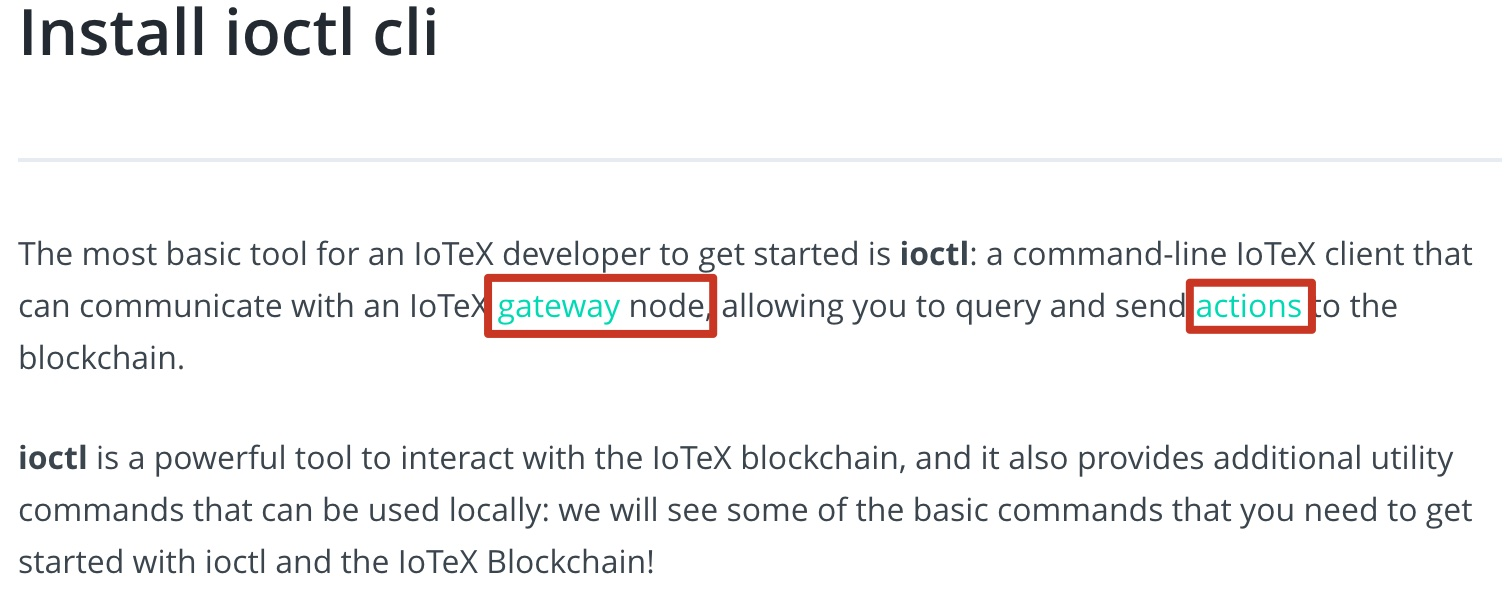
\includegraphics[width=8.33333in,height=\textheight]{images/install_cli.jpg}

Here you introduce the IoTeX \textbf{\emph{gateway}} node, and you
explain that it allows users to query and send \textbf{\emph{actions}}
to the blockchain, but I don't like how it links to that information
separately. I believe here you should actually explain what a gateway
and what an action is directly rather than linking to the definition
separately. And, \textbf{very importantly}, these hyperlinks are
\textbf{BROKEN} and need fixing:

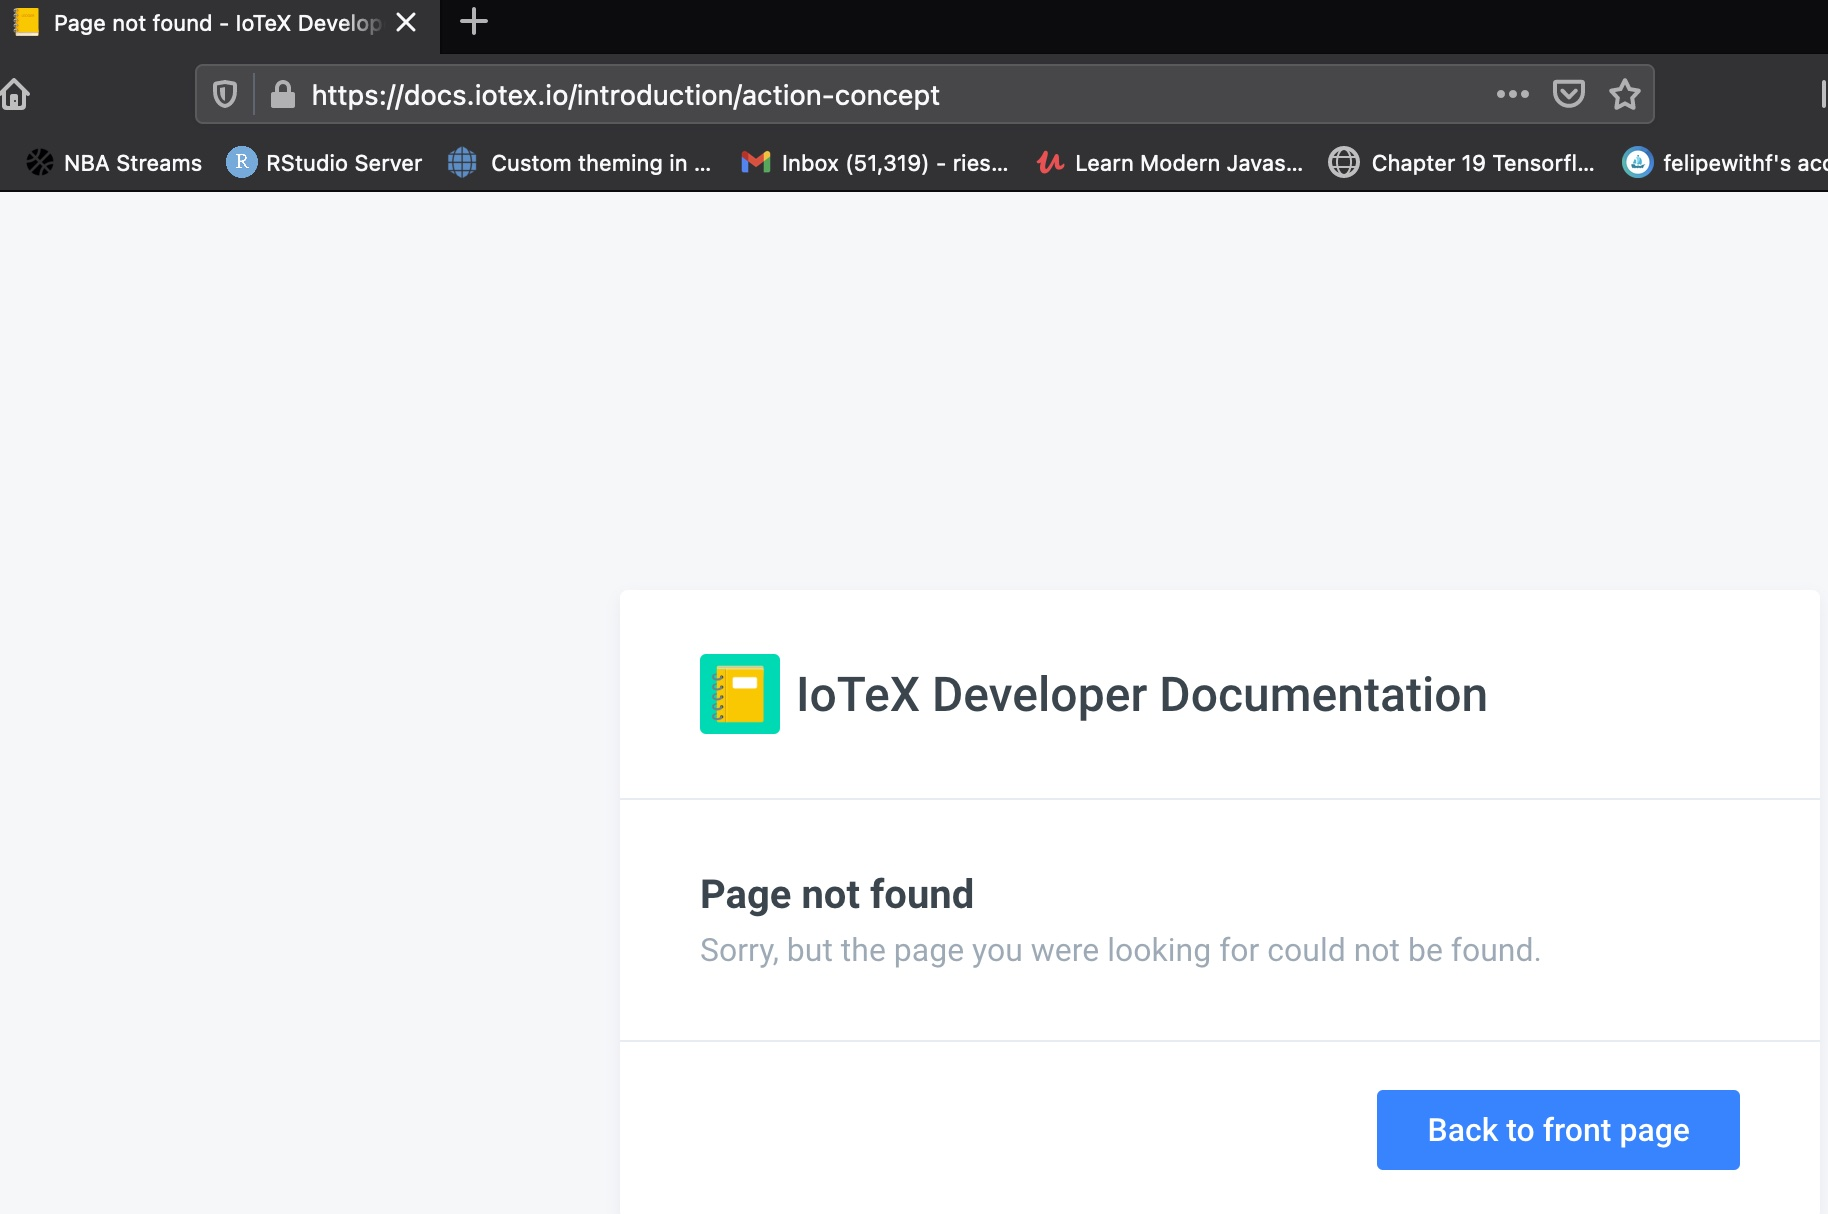
\includegraphics[width=7.29167in,height=\textheight]{images/actions_docs_not_found.jpg}

As of 05/27, the following two links are \textbf{both broken}:

\begin{itemize}
\item
  \url{https://docs.iotex.io/introduction/node-concept}
\item
  \url{https://docs.iotex.io/introduction/action-concept}
\end{itemize}

\hypertarget{usage}{%
\subsection{Usage}\label{usage}}

The installation does not seem to work on my MacBook Air (M1, 2021)
because of its arm64 architecture:

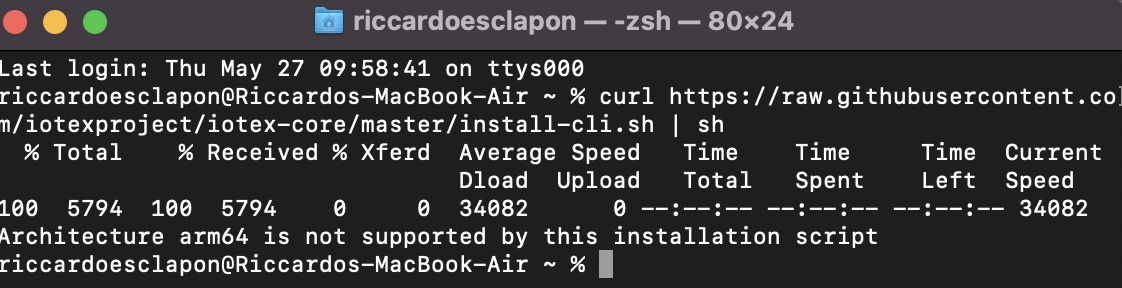
\includegraphics[width=7.29167in,height=\textheight]{images/install_cli_mac.jpg}

In my opinion it's going to present a challenge to a lot of people the
fact that this won't work on any new Mac products since late 2020 on the
M1 chip. For real adoption would be better to have more options than
just Linux.

I also think the link to the reference for the cli is useful, but having
it right below the step makes it seem like the next step. When going
through this, I instinctively clicked on that link for the next chapter
but was brought to the middle of nowhere in the references and was
confusing:

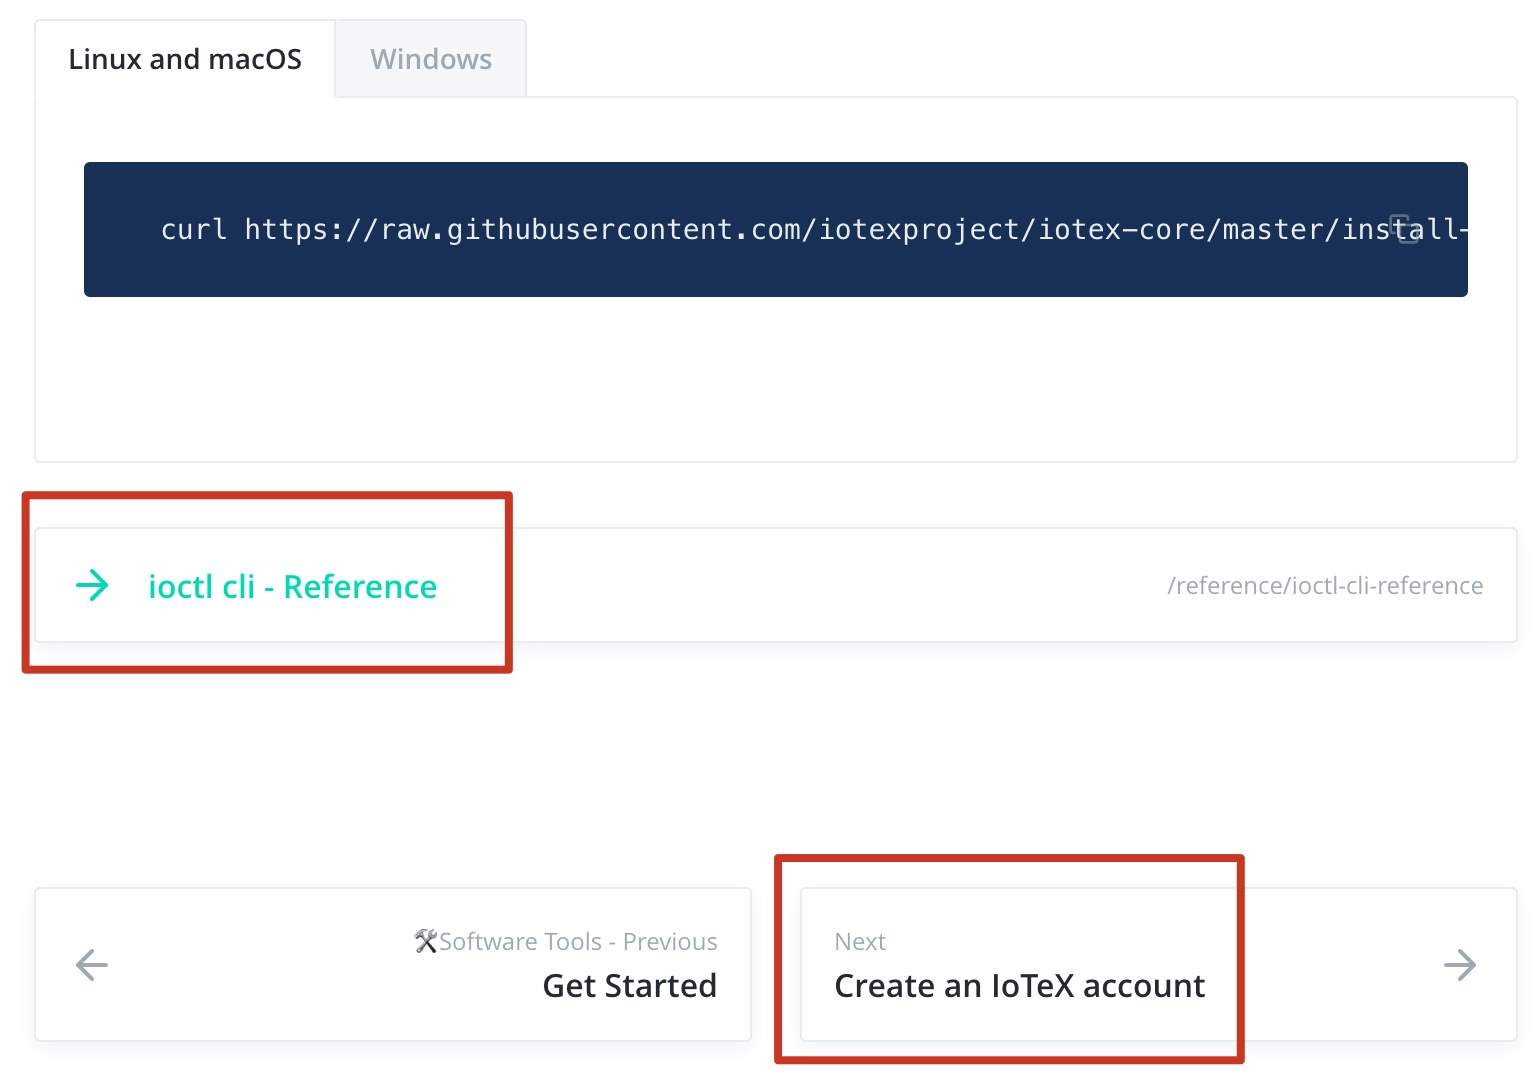
\includegraphics[width=7.29167in,height=\textheight]{images/install_cli_next.jpg}

\hypertarget{linux-install}{%
\subsubsection{Linux install}\label{linux-install}}

On Linux the installation worked as expected:

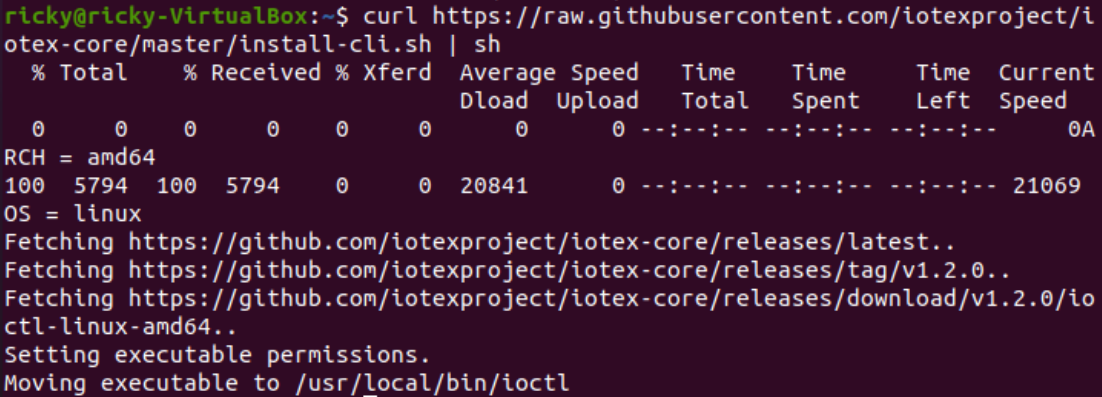
\includegraphics{images/linux_cli_install.PNG}

\hypertarget{create-an-iotex-account}{%
\section{Create an IoTeX account}\label{create-an-iotex-account}}

Broken hyperlinks circled below:

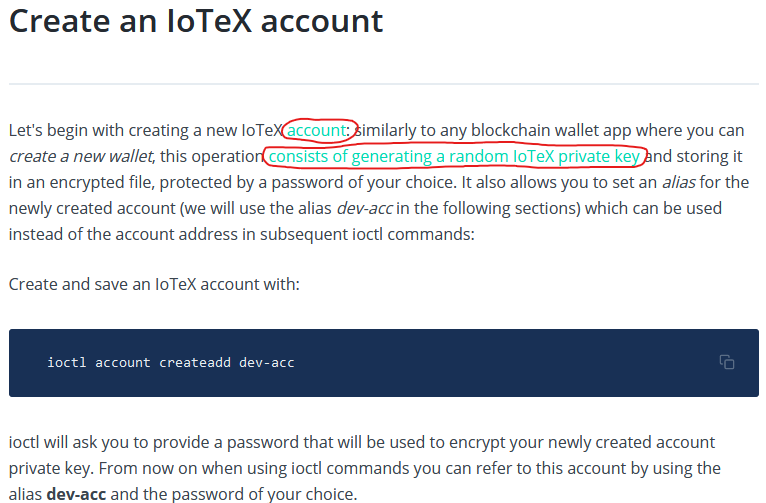
\includegraphics{images/create_iotex_account.png}

This command is supposed to prompt me to choose a password, but nothing
seems to happen on my end:

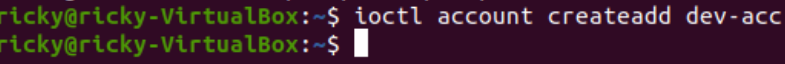
\includegraphics{images/create_account.png}

I watched the video embedded at the bottom of the page \textbf{\emph{An
introductory video to ioctl accounts management}} and followed the steps
as shown.

Running \texttt{ioctl\ account\ create}, still doesn't return anything:
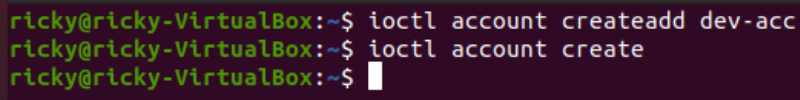
\includegraphics{images/create_account_video.png}

I also think it's odd that the video overview walks people how to do it
on Windows, but according to the documentations this does not currently
work on Windows. I tried the steps in the video and I can confirm it
does not work on Windows and powershell:

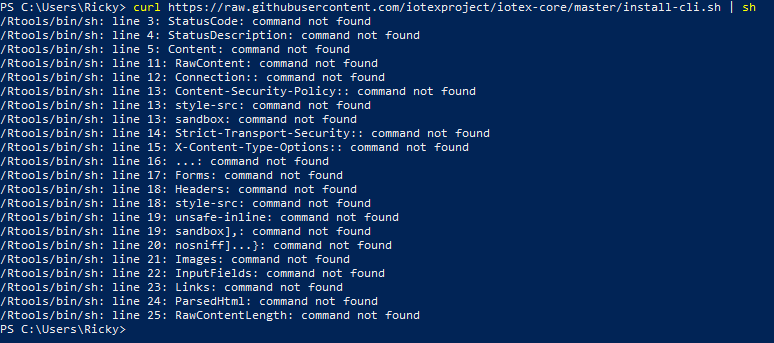
\includegraphics{images/windows_install_powershell.PNG}

The video is really good, but no commands seem to work on my end, but I
see nothing:

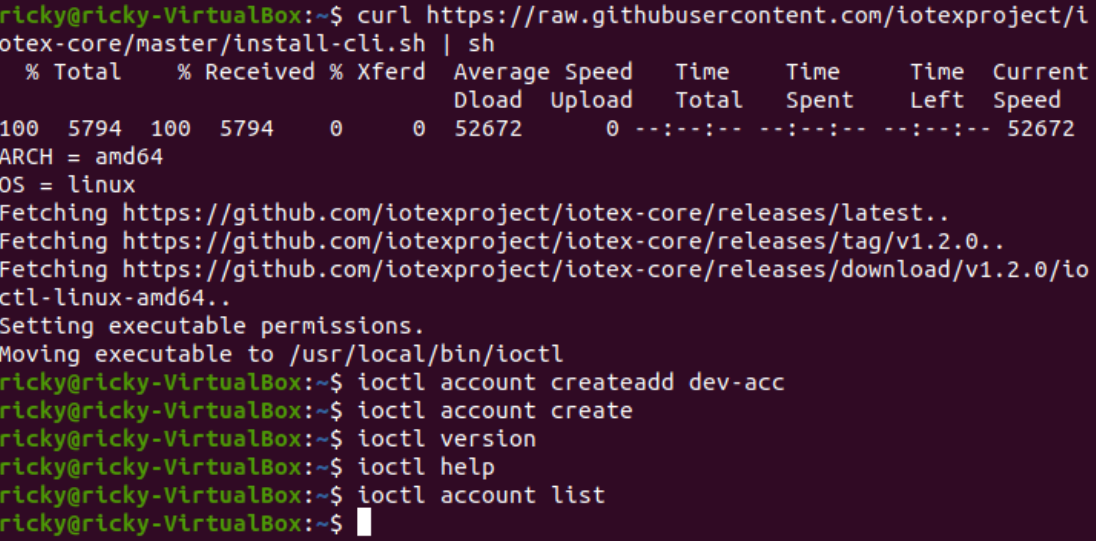
\includegraphics{images/linux_not_working.png}

\hypertarget{install-a-local-testnet}{%
\section{Install a local Testnet}\label{install-a-local-testnet}}

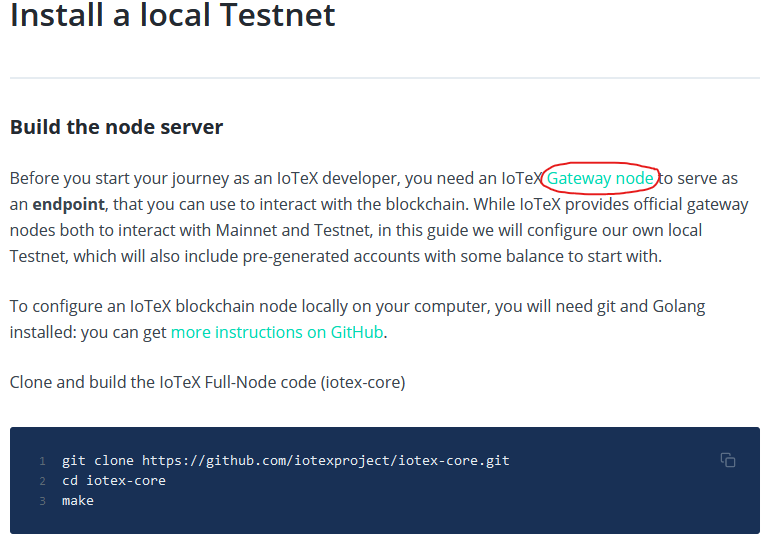
\includegraphics{images/install_local_testnet.PNG}

The link to the \textbf{\emph{Gateway node}} circled above is broken.

Following the commands in this section, this is what I get:

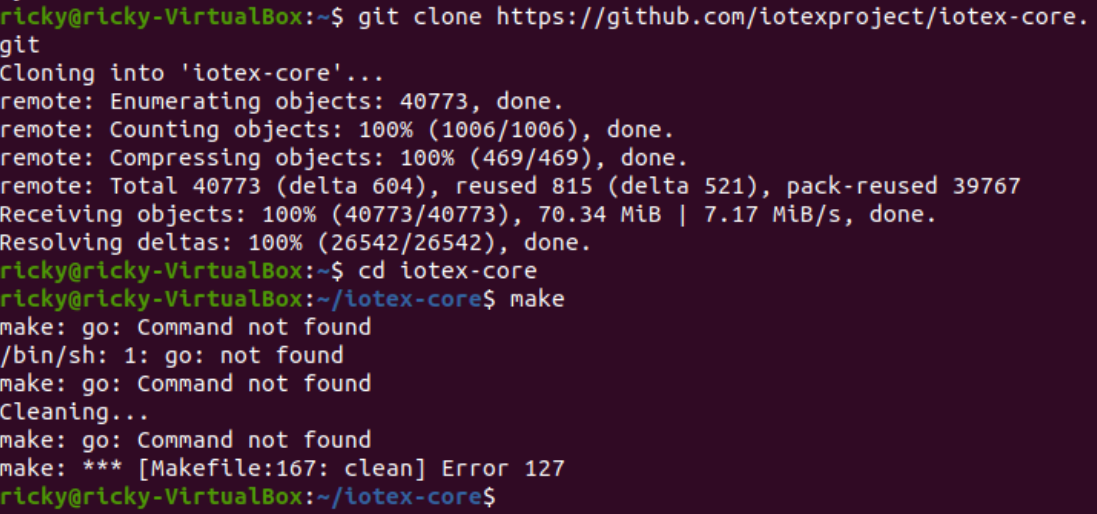
\includegraphics{images/testnet_git_problem.PNG}

After understanding the error I figured I did not have golang installed
on my machine. I was able to resolve the issue by installing golang with
\texttt{sudo\ apt\ install\ golang}. After running this command I no
longer get the previous error, but \textbf{it still does not work}:

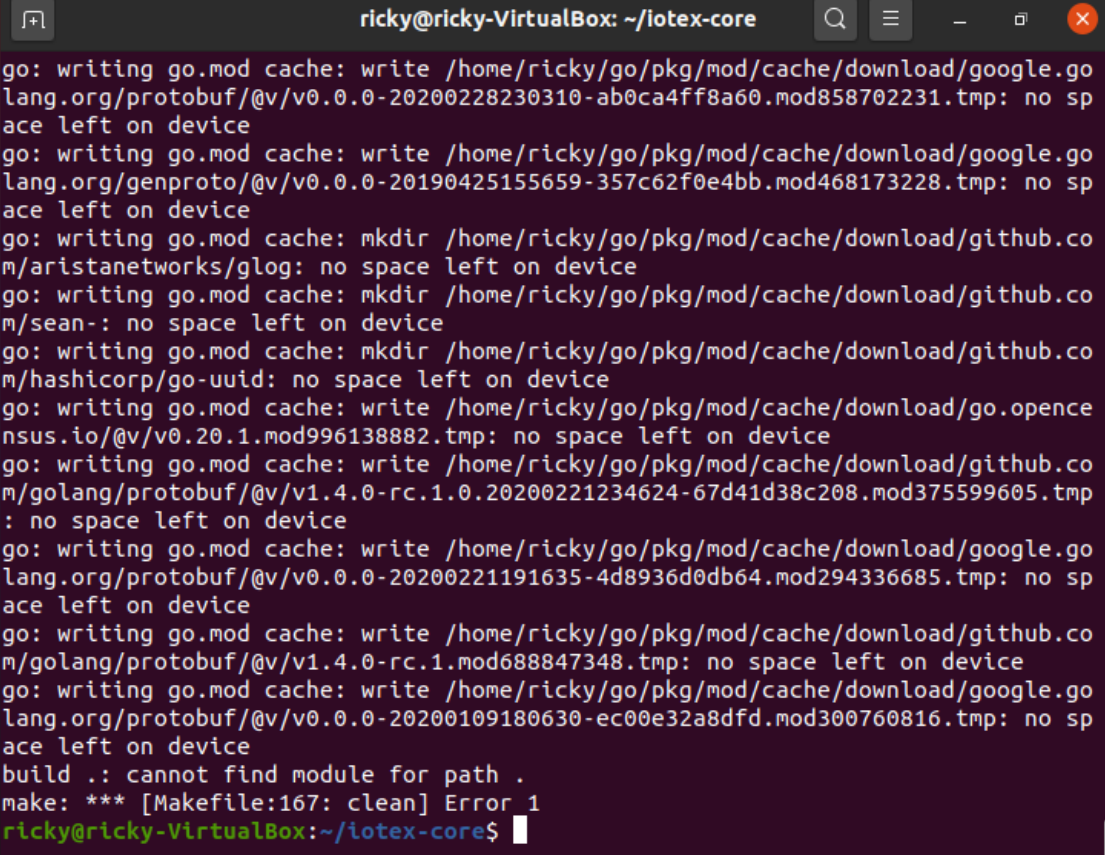
\includegraphics{images/make_error.PNG}

Looking through the GitHub repository, I noticed that golang was listed
as a dependency, and so was Protoc:

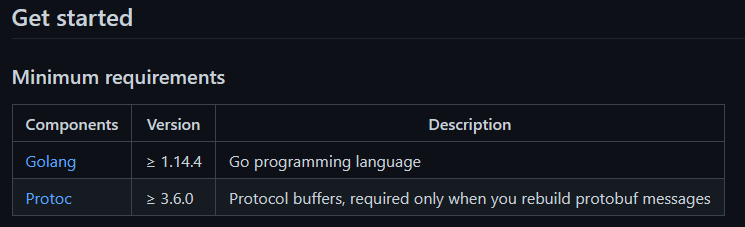
\includegraphics{images/requirements.PNG}

After a bit of digging I found the
\texttt{sudo\ apt\ install\ protobuf-compiler} worked to install the
other component I was missing. I think the error shown in the previous
screenshot \textbf{\emph{cannot find module for path .}} could be more
clear to instruct the user on what is missing and how to install the
missing component.

This time it ran for much longer and I got a different error:

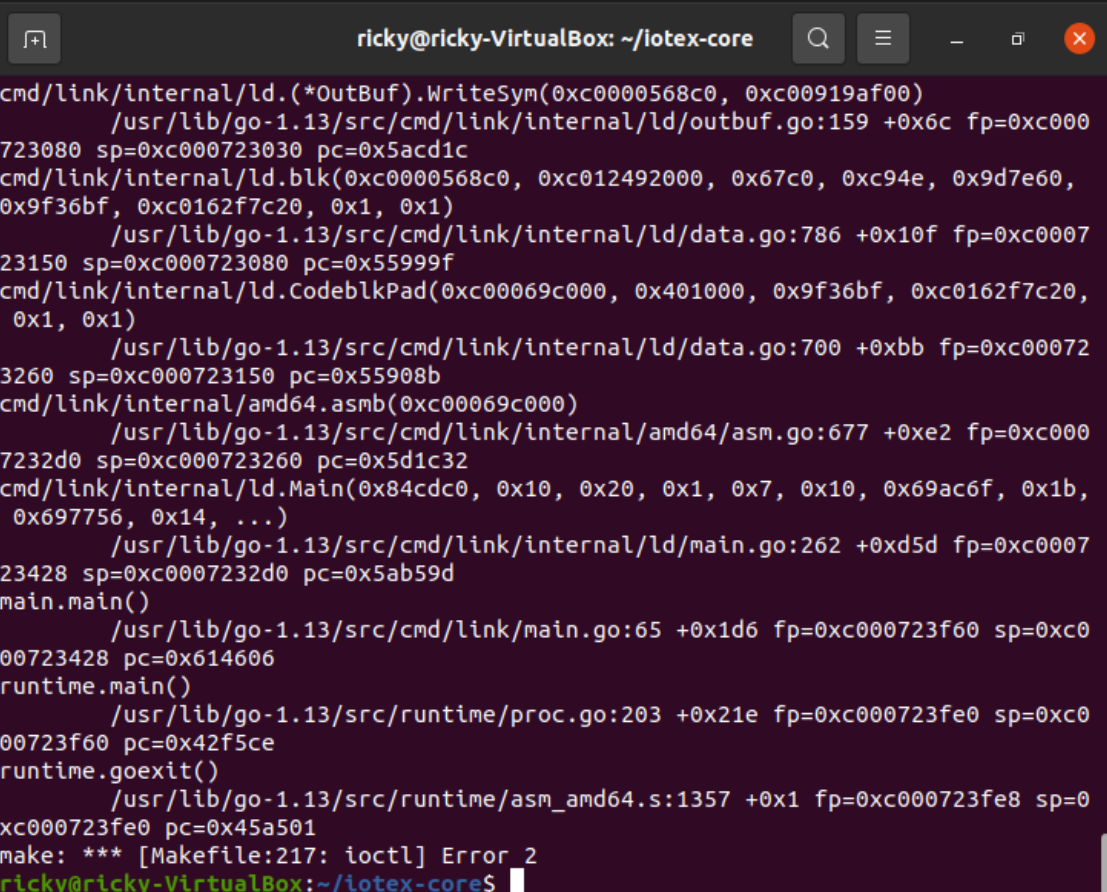
\includegraphics{images/protoc_error.PNG}

So this time I figured there was some kind of issue with ioctl since my
commands were not functioning as expected. After a lot of
experimentation I figured out that I needed to set an endpoint, and the
commands like \texttt{ioctl\ version} started finally working:

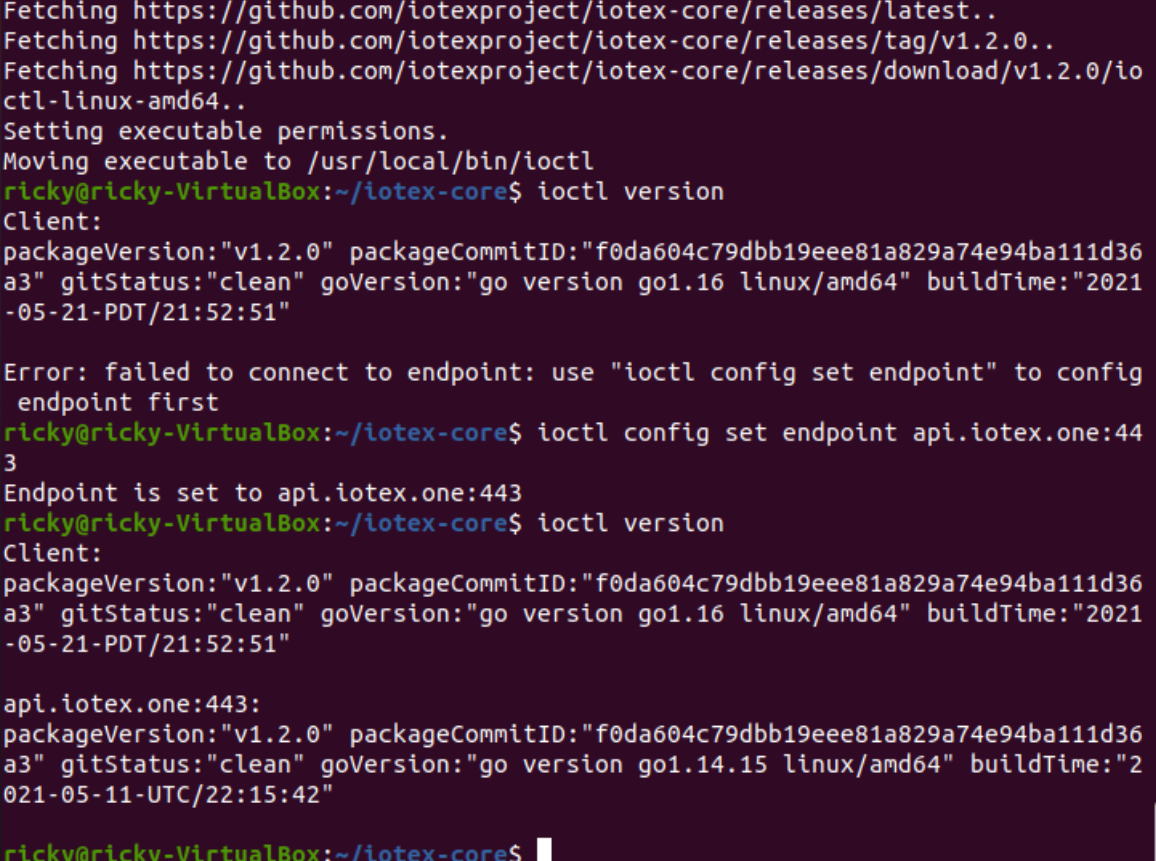
\includegraphics{images/linux_set_endpoint.PNG}

So \textbf{finally} I was able to follow along with the tutorial step of
\texttt{ioctl\ account\ createadd\ dev-acc}

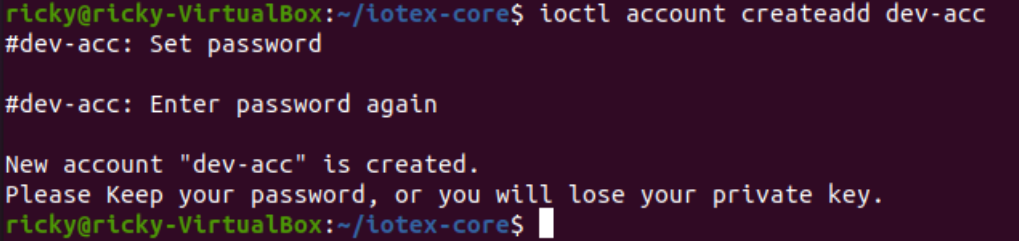
\includegraphics{images/create_account_works.PNG}

And all the commands that weren't doing anying before now seem to work
as expected:

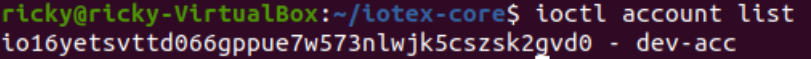
\includegraphics{images/list_accounts.PNG}

This time, when I run the \texttt{make} command, \textbf{\emph{yet
another error}}:

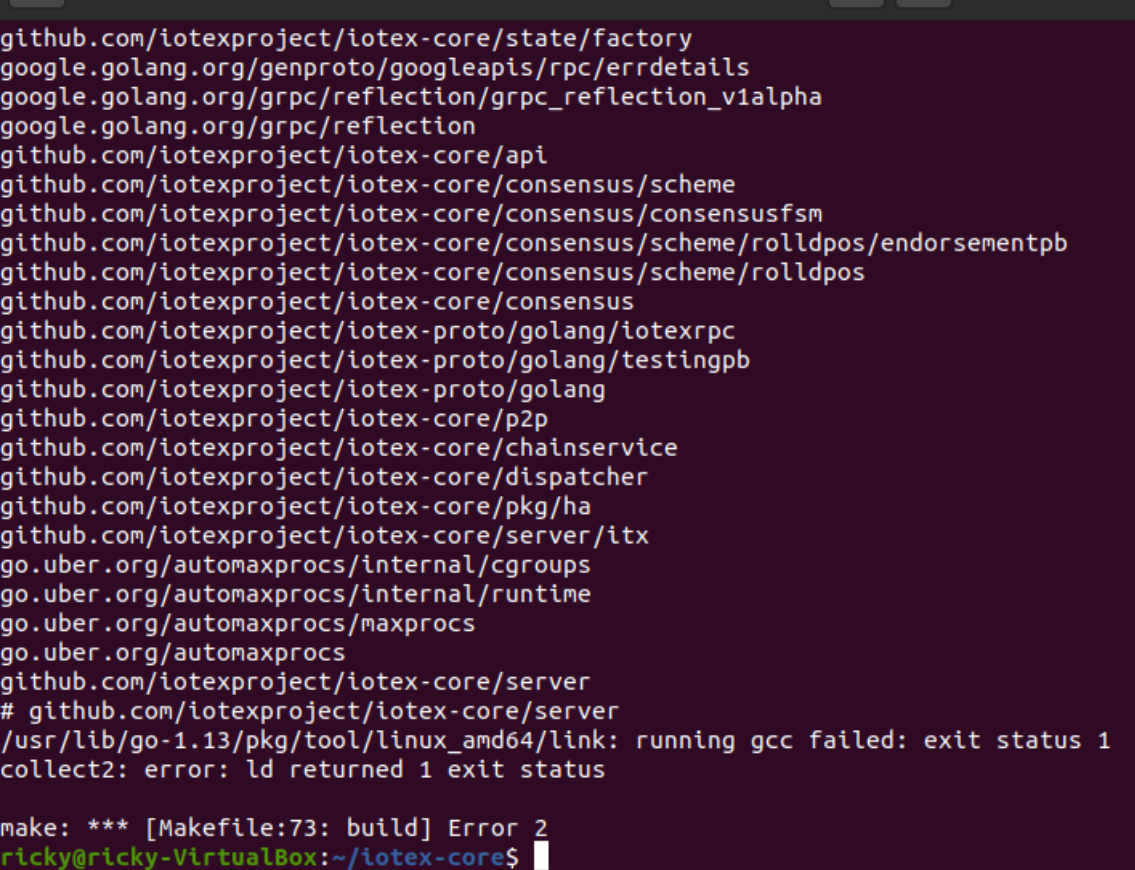
\includegraphics{images/linux_testnet_error.PNG}

Here is the best explanation I was able to find for this error:

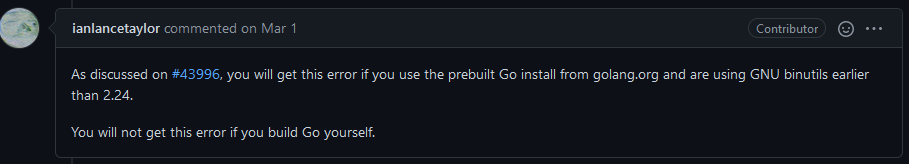
\includegraphics{images/golang_error.PNG}

At this point I called it quits, way too many errors, the
\href{https://docs.iotex.io/software-tools/get-started/install-ioctl-cli}{step
of \textbf{\emph{Install ioctl cli}}} for sure needs some more work in
my opinion. See section below.

\hypertarget{feedback---user-experience}{%
\section{Feedback - User Experience}\label{feedback---user-experience}}

This section was a bad experience on my end. Took me several hours to
just run to create the account through ioctl. Two things that would have
saved me all that time:

\begin{enumerate}
\def\labelenumi{\arabic{enumi}.}
\item
  Make the dependencies of Go and Protoc more obvious, and provide users
  with the installation commands for both as part of the tutorial
  (highlighted as an optional task if the user already has them
  installed).
\item
  The tutorial \textbf{\emph{NEEDS}} the command
  \texttt{ioctl\ config\ set\ endpoint\ api.iotex.one:443} in order to
  work. Without this step, on my end nothing was working at all, and
  worse it was just not returning any message at all, so it's impossible
  to debug.
\item
  More specific errors are needed. If you don't have a specific
  dependency of either Go or Protoc installed, the terminal should
  explicitly say so instead of returning a more ambiguous message. Only
  so much can be missing on the user's end, so it would be better to
  catch those specific circumstances.
\end{enumerate}

\hypertarget{interact-with-the-blockchain}{%
\section{Interact with the
blockchain}\label{interact-with-the-blockchain}}

I tried following the rest of the steps, but because of the issue
outlined up to this point, I was not able to follow along with the rest
of the steps:

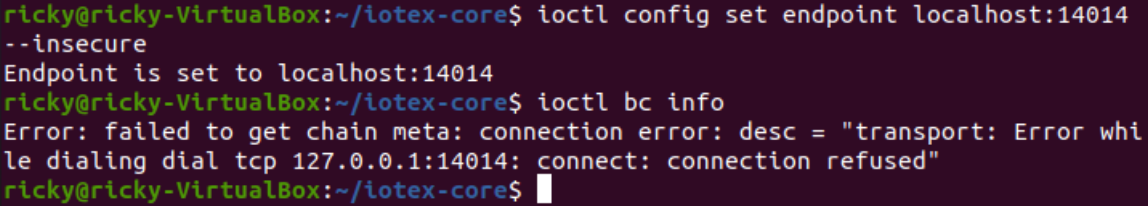
\includegraphics{images/interact_error.PNG}

\hypertarget{iotx-faucets}{%
\section{IOTX Faucets}\label{iotx-faucets}}

This step was a bit odd on my end. On my MacBook I ran into issues on
both Chrome and Firefox and the Google login works great, but when I
click ``Submit'', something was going wrong there. See error in top
right corner here:

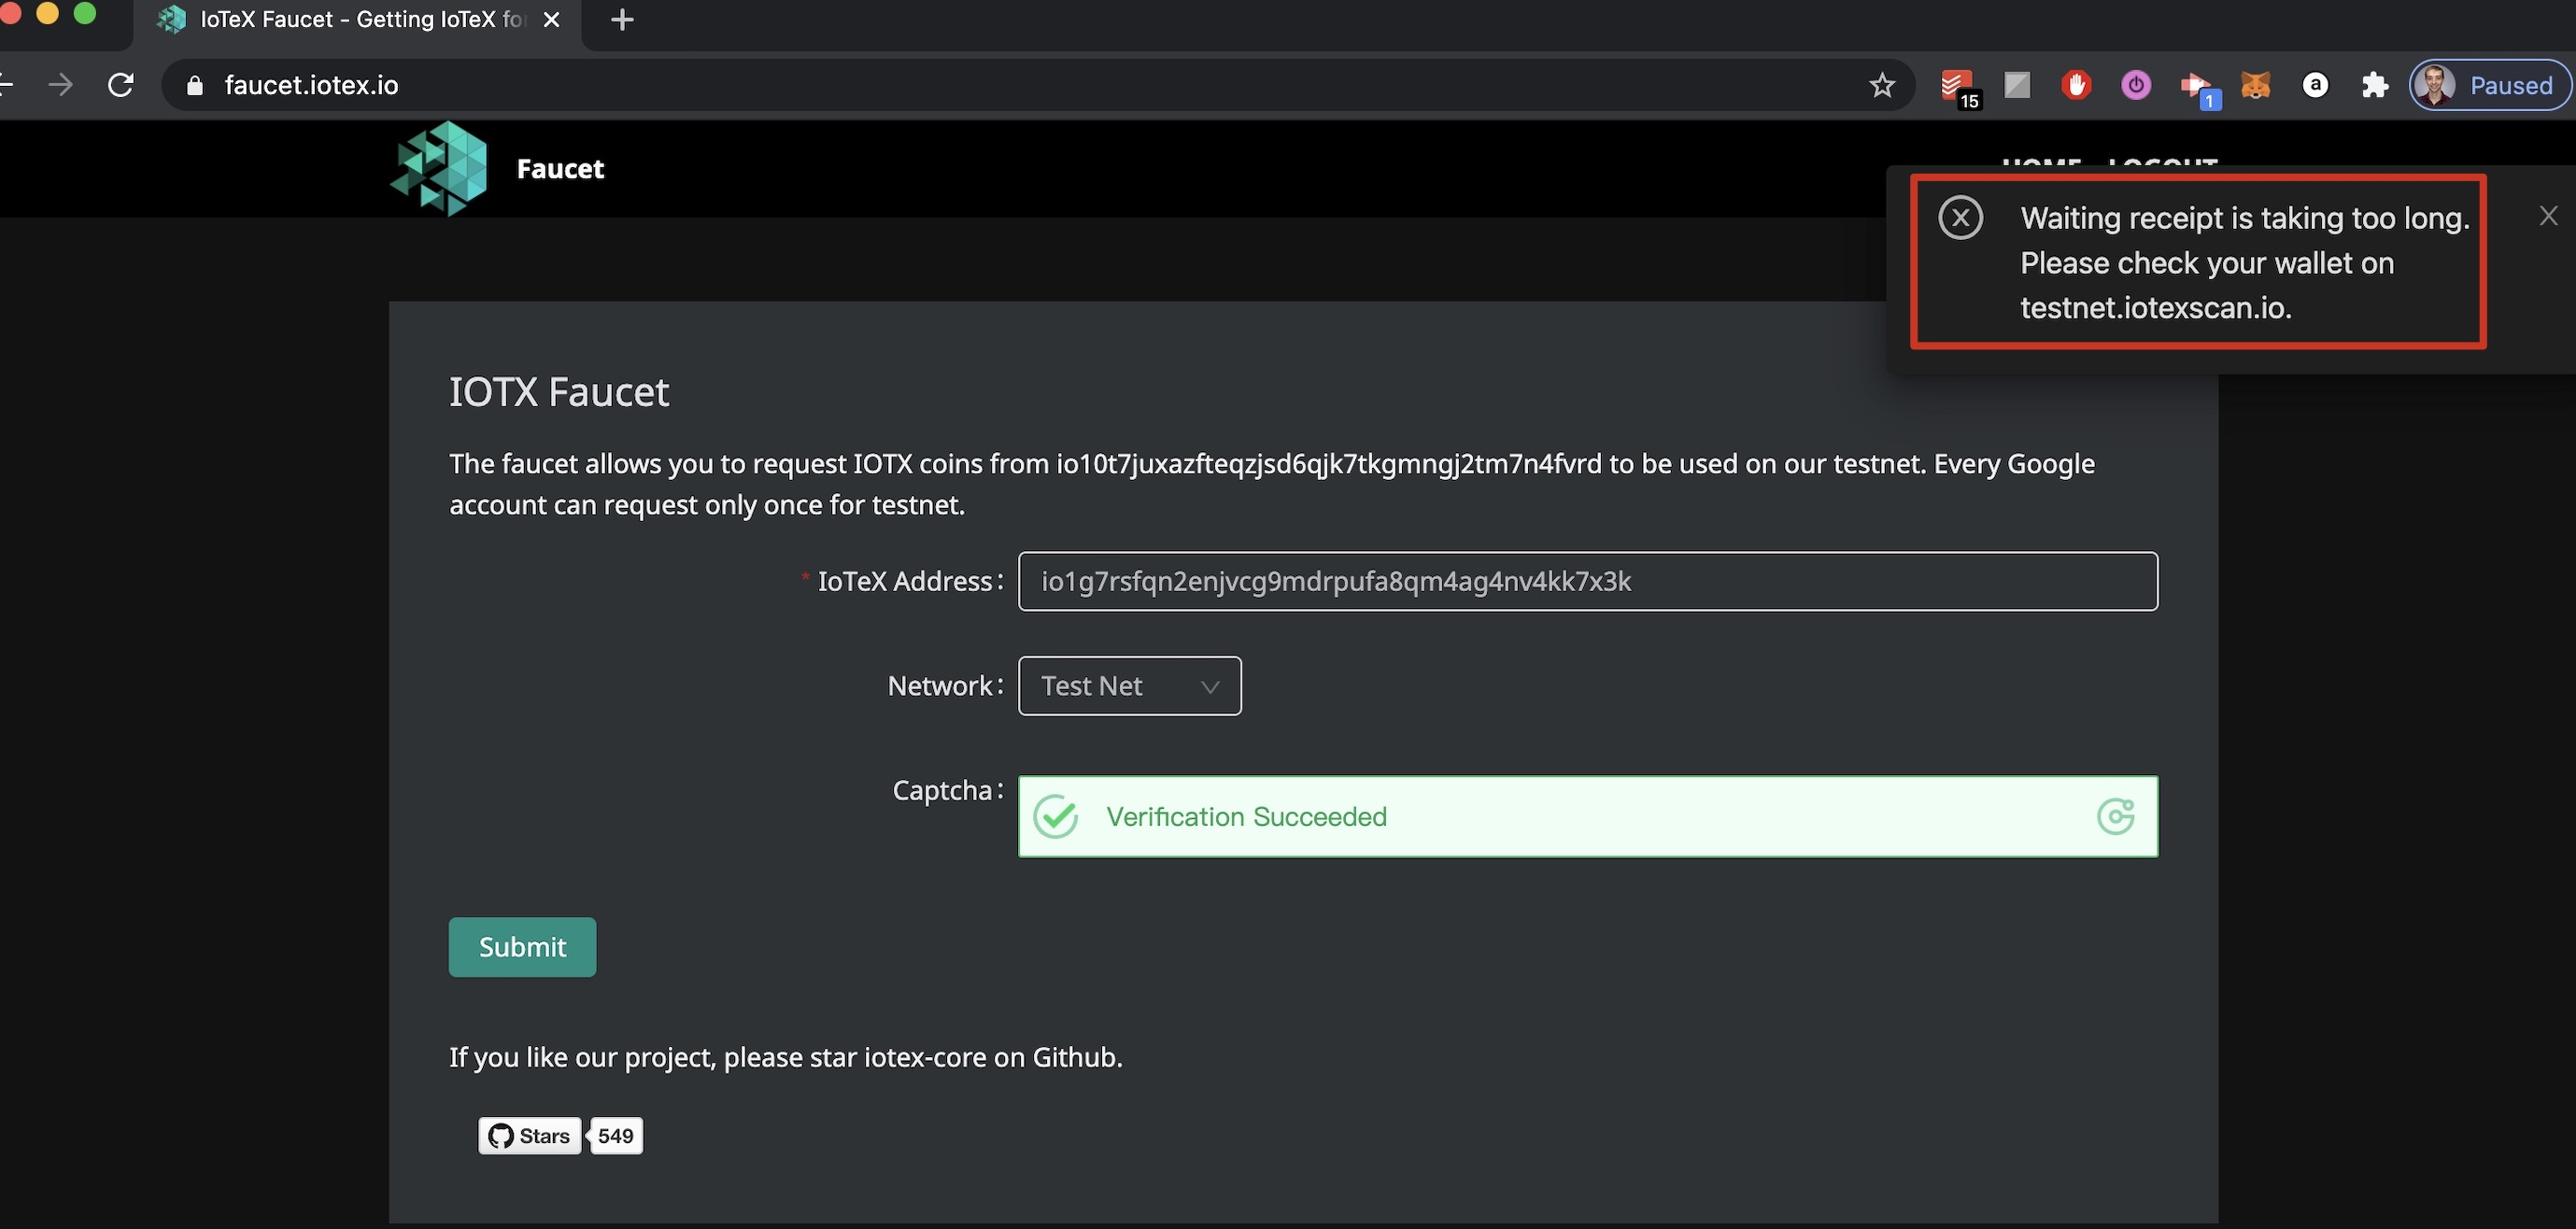
\includegraphics{images/iotex_faucet.jpg}

Doing it through my Linux environment on Firefox two days later worked
great:

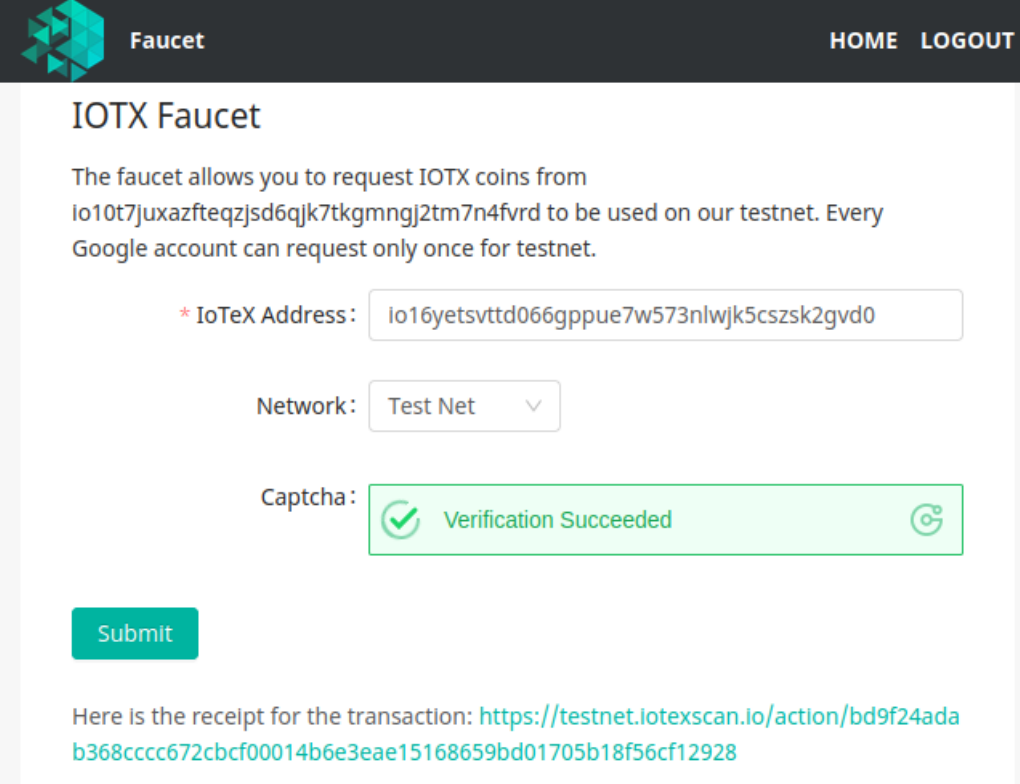
\includegraphics{images/iotx_faucet.PNG}

And the transaction hash and everything here looks great and correct:

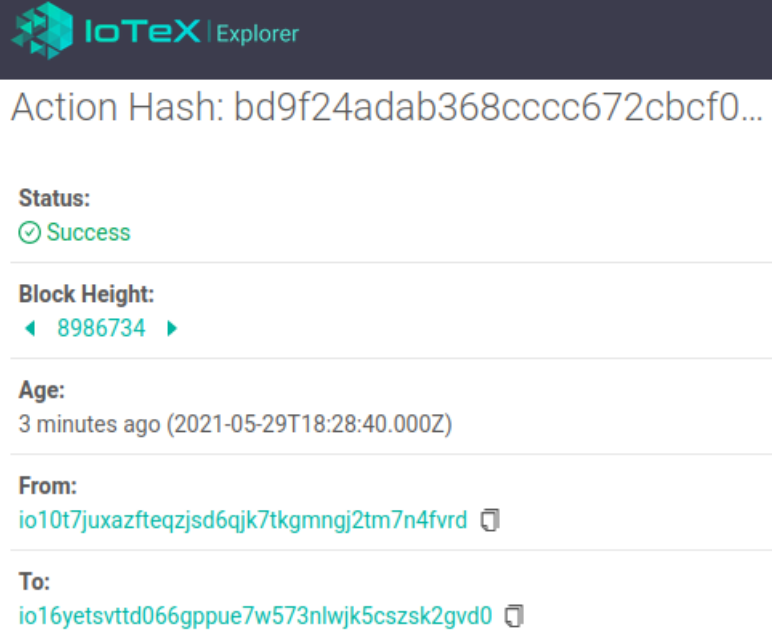
\includegraphics{images/transaction_explorer.PNG}

\hypertarget{note}{%
\subsubsection{Note}\label{note}}

One more quick observation here too is that faucet.iotex.io does not
automatically redirect a user to \url{https://faucet.iotex.io} which I
think would be good practice:


\includegraphics{images/unsecured_faucet.PNG}

\hypertarget{smart-contracts}{%
\chapter{Smart Contracts}\label{smart-contracts}}

\hypertarget{introduction-1}{%
\section{Introduction}\label{introduction-1}}

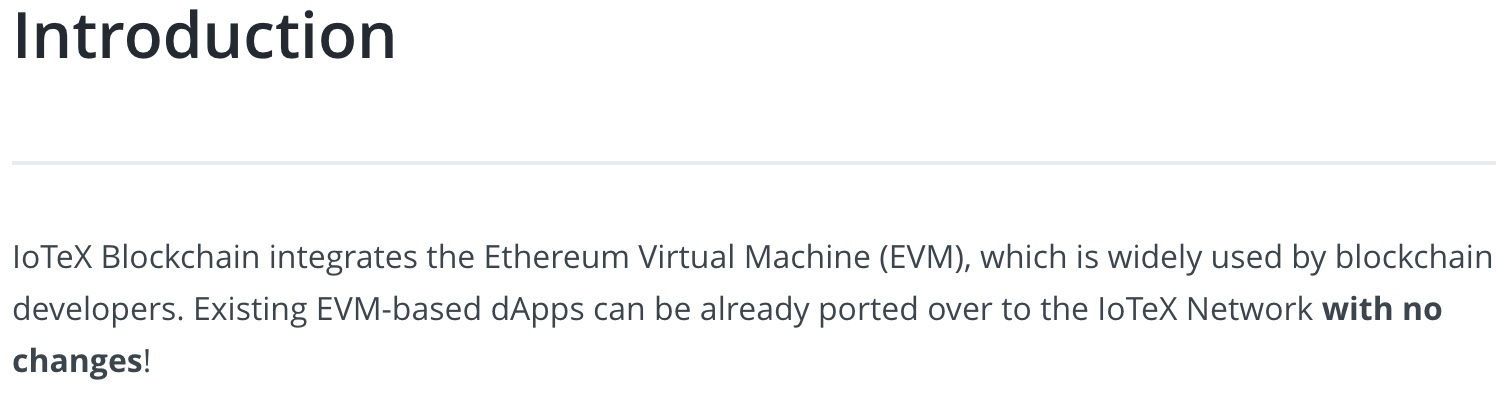
\includegraphics{images/smart_contracts_intro.jpg}

Here might be good to give a really basic understanding of what the EVM
is, or at least link to a resource for users to learn more.

\hypertarget{solidity-programming-language}{%
\subsection{Solidity Programming
Language}\label{solidity-programming-language}}

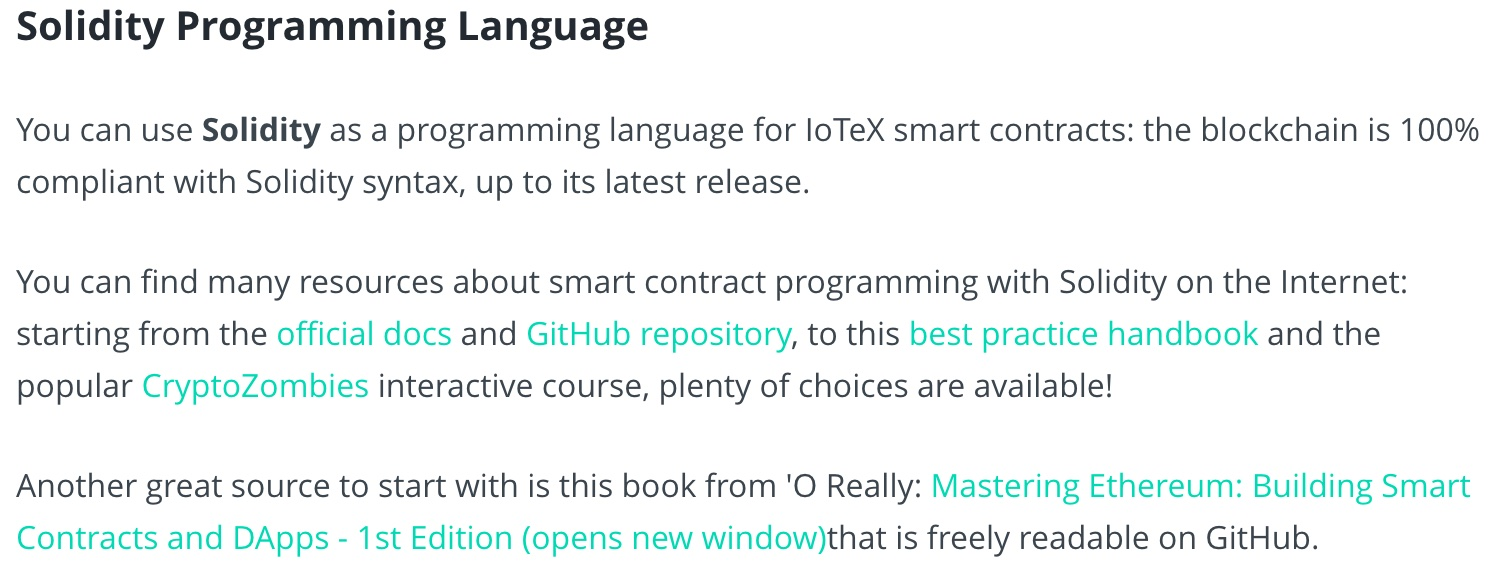
\includegraphics{images/solidity_programming_language.jpg}

Some great links in here and none of them are broken, so all good on
that front. One thing that caused some confusion for me was the sentence
\textbf{\emph{``compliant with Solidity syntax, up to its latest
release.''}}. Does this mean it's compliant up to the current latest
release (which one?), or does it mean that it will
\textbf{\emph{always}} be compliant with the latest release of Solidity?

The one thing that stands out to me here is that there isn't a very
strong introduction around smart contracts, what they actually do, and
why they are important. I think just one or two sentences around a smart
contract being a way to trust that a protocol will work the way its
supposed to work and a quick comparison between this mechanism and how
traditional companies work would be really helpful here before you start
talking about the specifics of solidity. Might also be worth verbalizing
better the connection between the EVM and the Solidity language, and how
other smart contract languages exist too.

\hypertarget{advantages-of-iotex-smart-contracts}{%
\subsection{Advantages of IoTeX Smart
Contracts}\label{advantages-of-iotex-smart-contracts}}

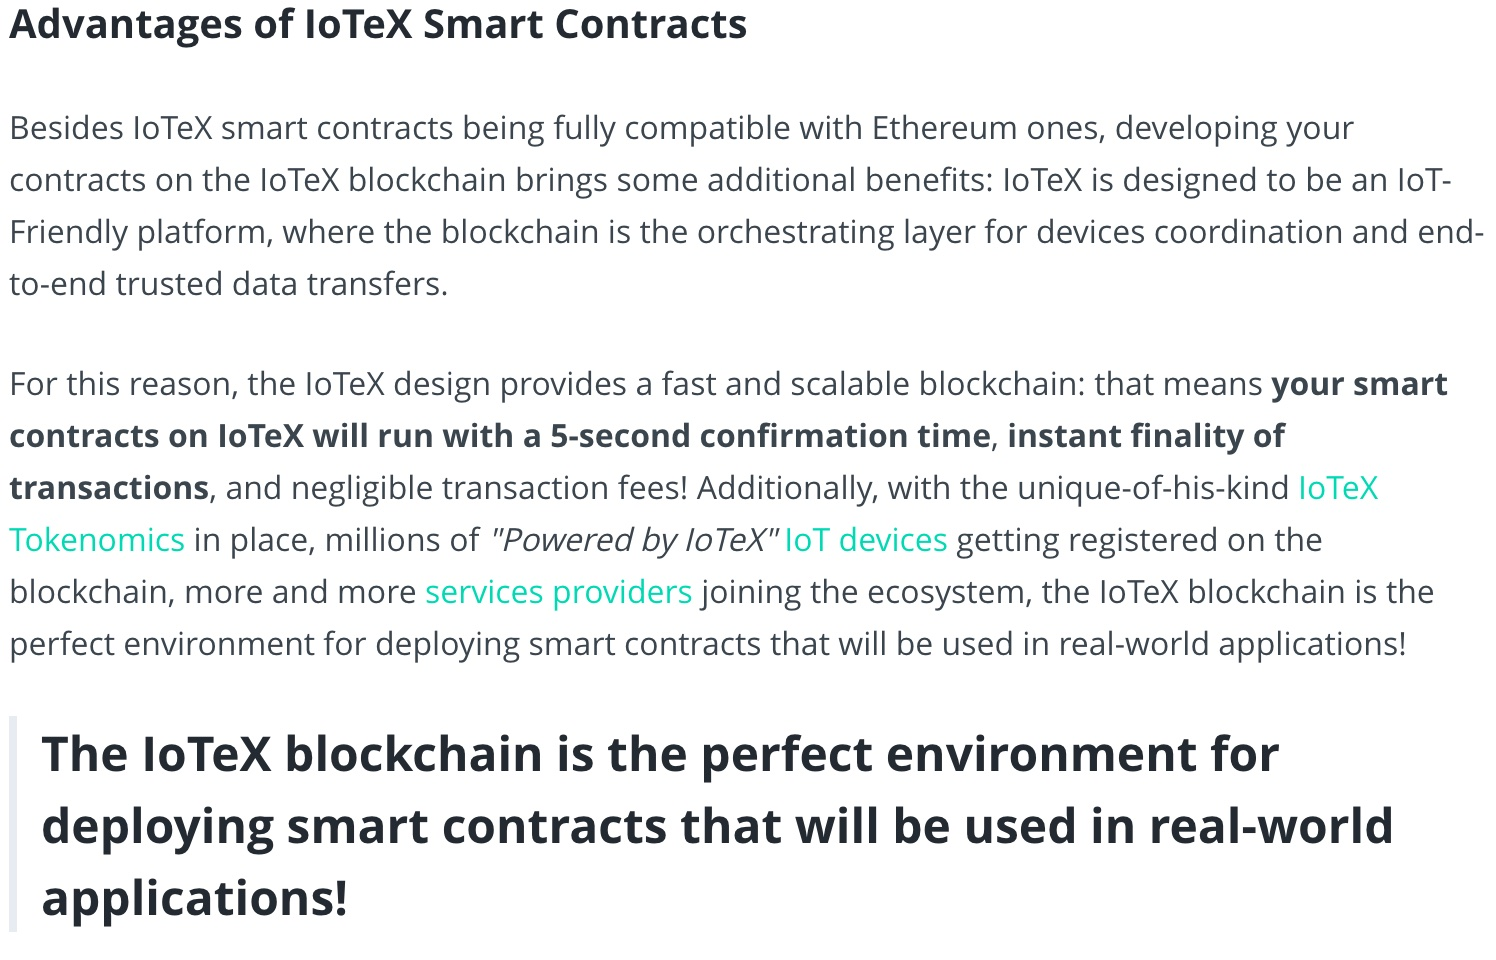
\includegraphics{images/advantages_smart_contracts.jpg}

This section is informative, but I think it should have a link/resource
added to it around \textbf{\emph{Roll-DPoS}} and how that functions, I
think that would be more relevant than the tokenomics link. I think it's
a fundamentally important point to understand to truly grasp how you get
to 5-second confirmation time, instant finality, and close to \$0
transaction fees. And I think it would really drive your point home of
why the IoTeX blockchain is the perfect environment for deploying smart
contracts that will be used in real-world applications. But really cool
that IoTeX smart contracts are backward compatible with the EVM.

\hypertarget{issue-xrc20-tokens-on-iotex}{%
\section{Issue XRC20 Tokens on
IoTeX}\label{issue-xrc20-tokens-on-iotex}}

One first observation for this section is that the link goes to
\url{http://iopay.iotex.io/desktop/} when
\url{https://iopay.iotex.io/desktop/} seems like the better option.

Here I was not able to download on Linux, so I moved to run the IoTeX
Desktop Wallet from Windows instead. I was able to repeat the steps on
Windows and get funds on the Test Net inside my desktop wallet:

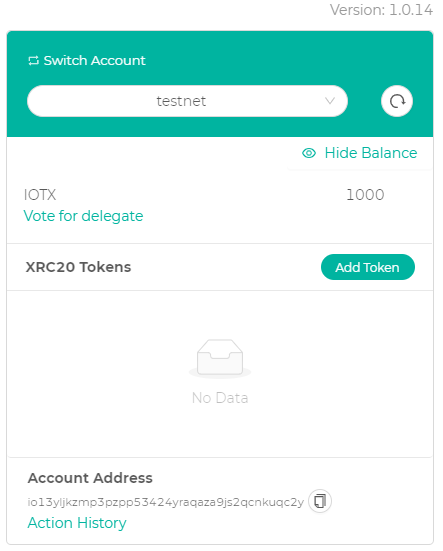
\includegraphics{images/desktop_funds.PNG}

\hypertarget{edit-solidity-code-in-iotex-studio-ide}{%
\subsection{Edit Solidity code in IoTeX Studio
IDE}\label{edit-solidity-code-in-iotex-studio-ide}}

I tried doing the steps outlined for ide.iotex.io, but when I click on
\textbf{\emph{Compile Contract}} absolutely nothing is happening (on
either environment of Javascript VM or deploy via ioPay). No clue what I
am doing wrong:

\includegraphics{images/ide_iotex_nothing.gif}

I tried from Mac, Windows, and Linux and could not get it to work on any
of them. Here is an example trying from Windows deploying the smart
contract to the ioPay Desktop environment:

\includegraphics{images/deploy_smart_contract_no_response.gif}

No clue what I'm doing wrong here. But in terms of feedback I think the
code in step 2 could optionally be explained in more detail. One idea
would be to explain what each step does in more detail through some type
of other separate link and be able to dig into each step (like
understanding the functionality of each of the three import statements
one by one). The code in the documentation looks good, but the code
linked on GitHub looks a bit off in terms of having the import link to
the proper url and not sure if it's importing from its own repository or
something:

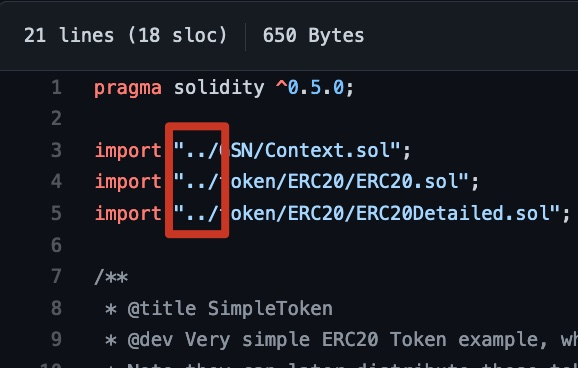
\includegraphics{images/github_token_paths.jpg}

Overall though I think the steps as they are outlined are very logical
and clear for this section, and it makes sense.

\hypertarget{note-1}{%
\subsection{Note}\label{note-1}}

As shown in the short videos embedded above, nothing was happening in
the ioPay Desktop app. About an hour later though I noticed that I did
have a prompt that \textbf{\emph{eventually}} showed up:

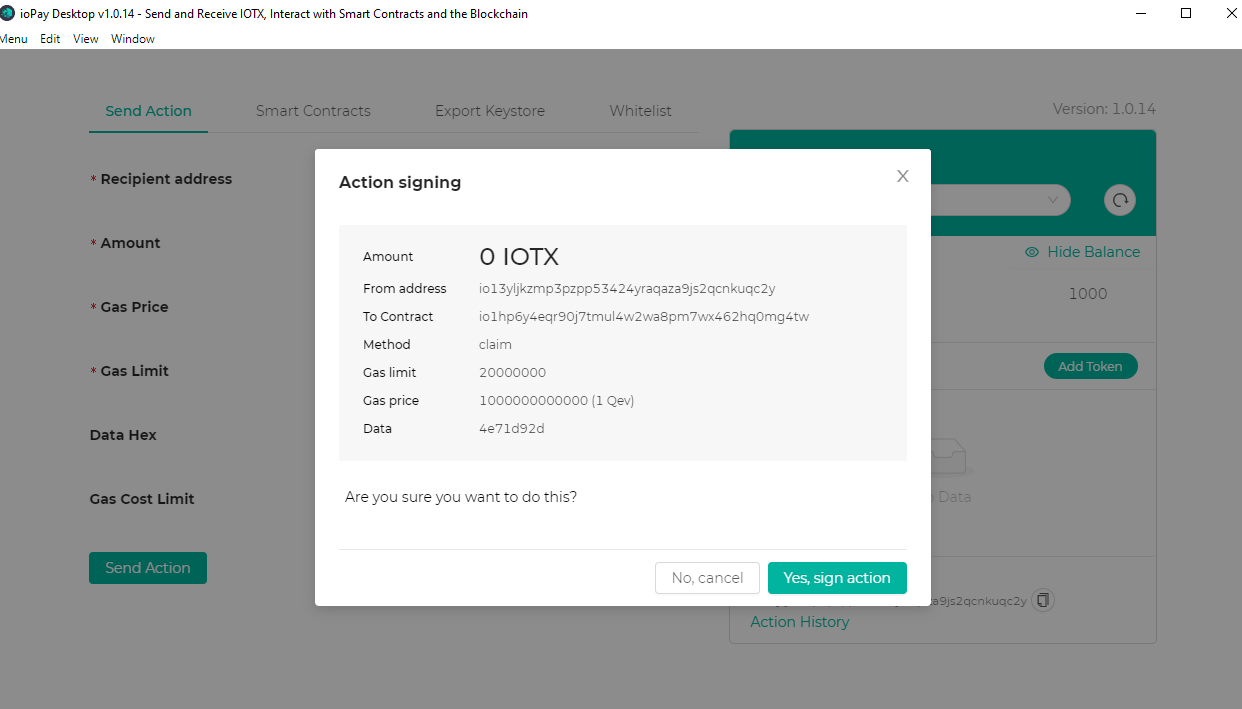
\includegraphics{images/desktop_prompt.PNG}

But I didn't have the website open anymore because it had been a long
time, and when I went back to ide.iotex.io I was not able to find the
compiled contract as shown in the last step of \textbf{\emph{3. Build
and Deploy}}.

\hypertarget{token-metadata}{%
\section{Token Metadata}\label{token-metadata}}

This section is clear, but I think the metadata itself could be
discussed more. I would almost like to see the JSON example from the
GitHub repository be added into the official docs and have more of a
discussion around what each one represents so people can get a better
understanding of what to change and when. I think most people would
figure out to change most of these, but would be great to give more
details around the \textbf{\emph{type}} (xrc20 vs.~xrc721 and linking to
good resources that give a good comparison of the two token standards),
as well as the \textbf{\emph{decimals}} and maybe giving a simple
example of choosing one option over another on those two.

But the
\href{https://github.com/iotexproject/iotex-token-metadata\#iotex-token-metadata}{GitHub
repository} is really great and the \textbf{\emph{New token submission
process}} is very clearly outlined and I have no questions around that
process, seems straightforward. The only question that comes to mind
here is if one could have their token arbitrarily be rejected (outside
of established guidelines). I also really like the code for the
\textbf{\emph{Usage}} section and how it's way simple code, that's
awesome.

\hypertarget{iotex-antenna-sdk}{%
\chapter{iotex-antenna SDK}\label{iotex-antenna-sdk}}

Good links here, but the link to \textbf{\emph{Examples}} still appears
to be empty:

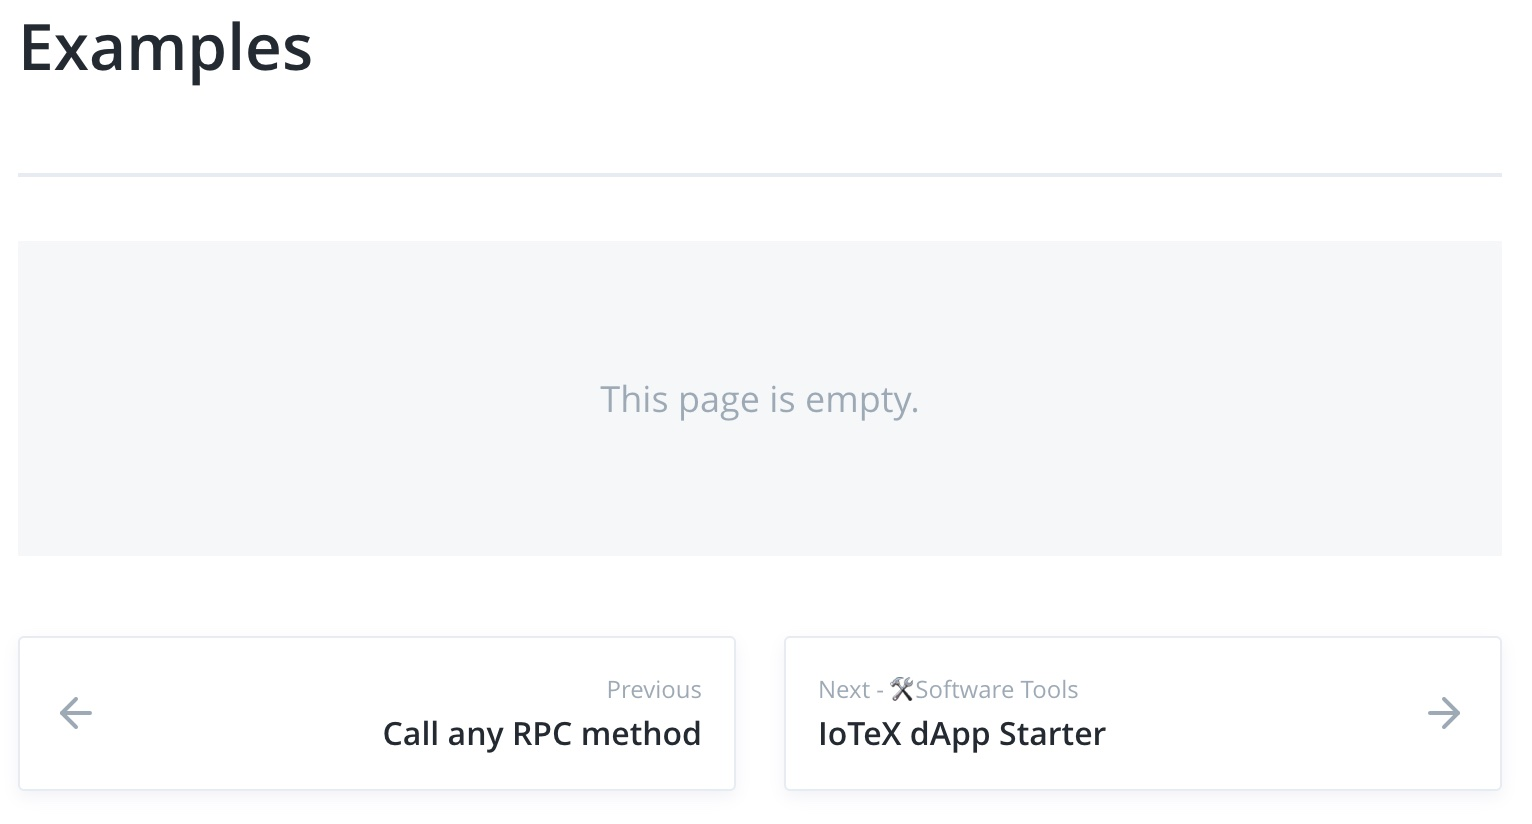
\includegraphics{images/antenna_SDK_examples.jpg}

\hypertarget{overview}{%
\section{Overview}\label{overview}}

Good informative overview. All links are functional. For the
\textbf{\emph{Reference implementation}} link might be good to bring to
the \textbf{\emph{Reference code}} section/homepage rather than the
\textbf{\emph{Create an account}} page specifically.

\hypertarget{installation}{%
\section{Installation}\label{installation}}

I followed the instructions for Antenna JS and did not run into problems
on install:

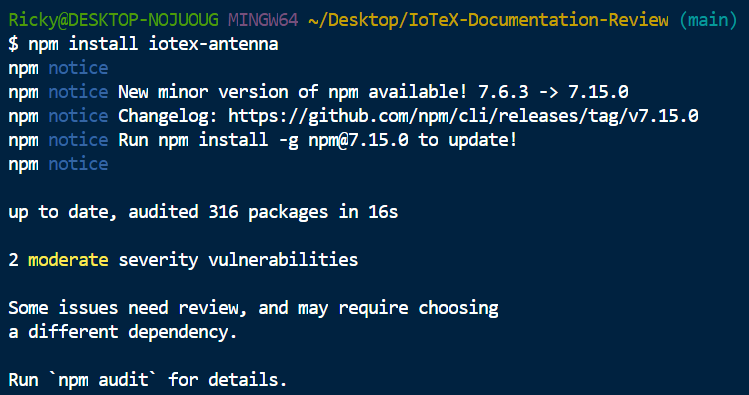
\includegraphics{images/install_antenna.PNG}

For this section I think it would be good if the ``Next'' button pointed
to the actual next steps the user should take with the antenna SDK,
bringing the user to the examples pace would be good.

\hypertarget{iotex-dapp-starter}{%
\chapter{IoTeX dapp starter}\label{iotex-dapp-starter}}

\hypertarget{deploy-on-heroku}{%
\section{Deploy on Heroku}\label{deploy-on-heroku}}

Did not run into any issues when deploying to Heroku. Had never used it
and made an account and worked really well out of the box just pressing
the button and following the prompt:

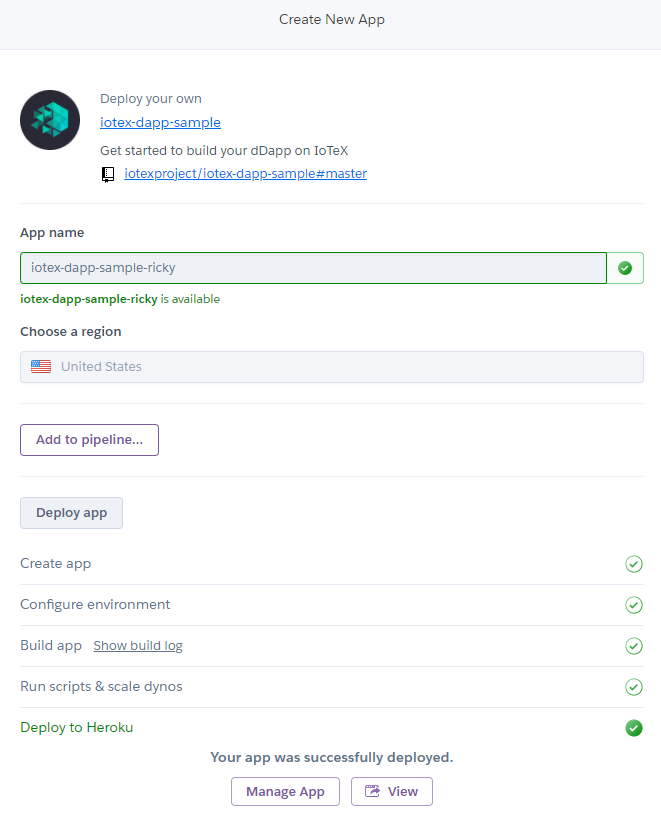
\includegraphics{images/heroku_deploy.PNG}

So no issues at all to get to the working dApp:

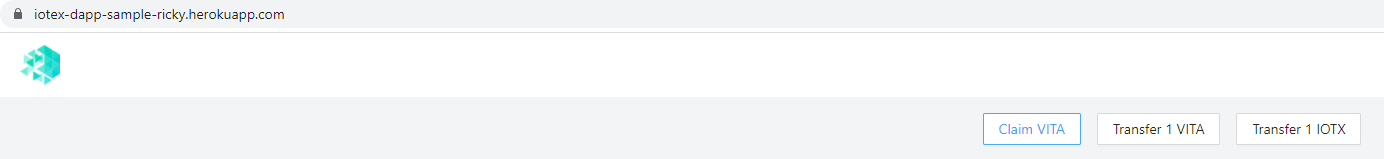
\includegraphics{images/heroku_app.PNG}

The only thing I'm not sure of is where one can find the actual files
that make everything work behind the scenes, but it's all available on
the \href{https://github.com/iotexproject/iotex-dapp-sample}{GitHub
repository} so that works well.

For this part:

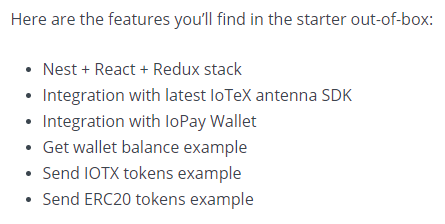
\includegraphics{images/dapp_starter_features.PNG}

This is really awesome, but would be even more awesome and functional if
each of these linked to a high-level explainer, even if that explainer
just re-directs to other pieces of the documentation where those topics
were discussed.

\hypertarget{middleware}{%
\chapter{Middleware}\label{middleware}}

Helpful guide on including the decentralized identity aspect into dApps
with helpful smart contract code snippets.

For \textbf{\emph{Security Considerations}} section, the hashtag
hyperlinks on the left side are broken.

\hypertarget{pebble-tracker}{%
\chapter{Pebble Tracker}\label{pebble-tracker}}

\hypertarget{quick-start}{%
\section{Quick Start}\label{quick-start}}

I don't own the device so I can't give a review of the quick-start
example, but I absolutely \textbf{love} this page. This is such an
impressive/awesome device, I might have to actually pre-order one for
myself. I watched some videos about it, and I don't really have any
feedback for this section, it's really clear and the dashboard is really
clear and impressive.

\hypertarget{technical-specification}{%
\section{Technical Specification}\label{technical-specification}}

None of these links work:

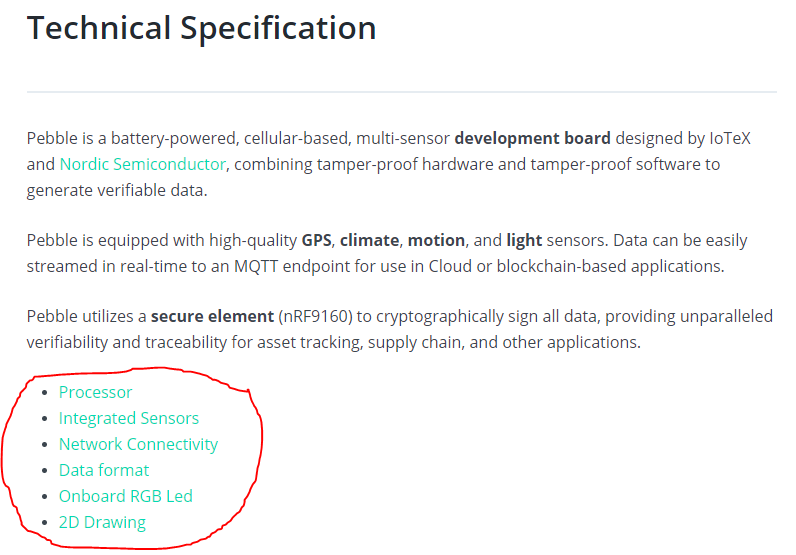
\includegraphics{images/technical_specification_missing_links.PNG}

Outside of that this page is great, I love how it outlines each sensor
with a link to the manufaturer, as well as having details around the
accuracy of each one, really nice. No complaints here.

\hypertarget{hardware-setup}{%
\section{Hardware Setup}\label{hardware-setup}}

Informative section, nicely polished and great labeled images of the
device.

The only link that seems to be broken here is the AT\&T link:


\includegraphics{images/att_404.PNG}

\hypertarget{setup-modes}{%
\section{Setup Modes}\label{setup-modes}}

No broken links here. Helpful overview of the difference between the two
modes, but would be great to learn more about the specifics around TLS
protecting the communications. But makes sense on when you should use
the different tech stacks.

I reviewed the instructions for both the Development mode and the
Production mode, and I did not find any broken links in these sections.
These sets of instructions here are really impressive! Really thorough,
well explained, and walks you through the whole step-by-step process, I
don't have any feedback on these ones, they look good.

\hypertarget{develop-and-build-the-firmware}{%
\section{Develop and Build the
Firmware}\label{develop-and-build-the-firmware}}

\hypertarget{build-on-windows}{%
\subsection{Build on Windows}\label{build-on-windows}}

All of these links appear to be broken currently:

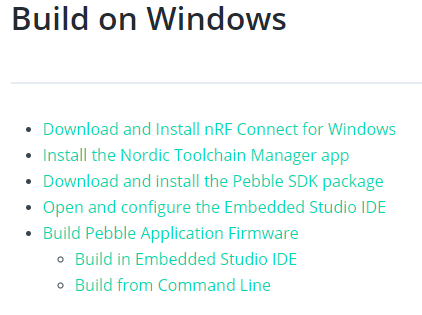
\includegraphics{images/build_windows_broken_links.PNG}

All other links on this page are good. These instructions make sense and
there are a lot of screenshots and it's pretty thorough, so this one
looks pretty good too.

\hypertarget{build-on-linuxmacos}{%
\subsection{Build on Linux/macOS}\label{build-on-linuxmacos}}

These links also appear to be broken:

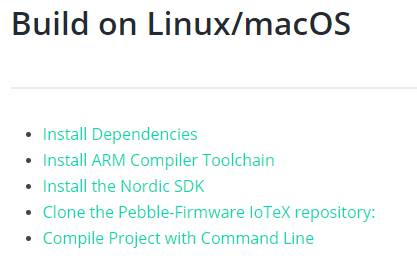
\includegraphics{images/build_linux_broken_links.PNG}

\hypertarget{configure-the-firmware}{%
\section{Configure the firmware}\label{configure-the-firmware}}

No comments/feedback for this section

\hypertarget{application-firmware}{%
\section{Application firmware}\label{application-firmware}}

No broken links, informative and well put together section.

\hypertarget{bootloader-firmware}{%
\section{Bootloader firmware}\label{bootloader-firmware}}

All good on this section with the exception of this broken link for
\textbf{\emph{Download the firmware}}:

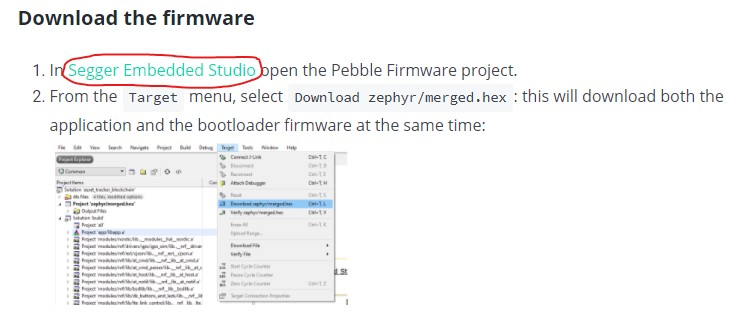
\includegraphics{images/download_firmware_link.jpg}

\hypertarget{more-resources}{%
\chapter{More Resources}\label{more-resources}}

\hypertarget{exchange-integration---general-guide}{%
\section{Exchange Integration - General
Guide}\label{exchange-integration---general-guide}}

Broken links highlighted below:

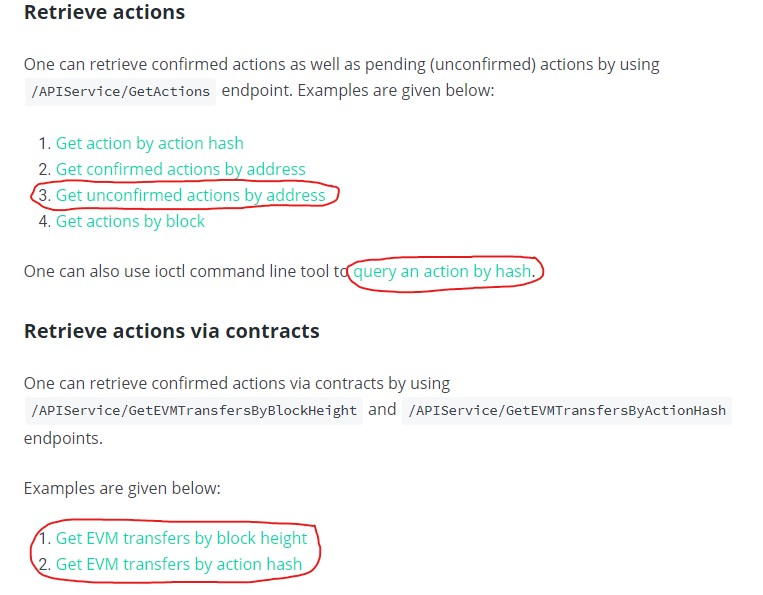
\includegraphics{images/retrieve_actions_link.jpg}

All other links seem good. Cool that there is documentation out there
for the exchanges to understand how to integrate with the IoTeX
blockchain.

\hypertarget{exchange-integration---rosetta-api}{%
\section{Exchange Integration - Rosetta
API}\label{exchange-integration---rosetta-api}}

This one seems all good, no broken links.

\hypertarget{action-injector}{%
\section{Action Injector}\label{action-injector}}

Really cool that one can simulate random action traffic, impressive
feature.

However, this \textbf{command does not work}. Tried on both Windows and
Linux and it failed on both.

\hypertarget{hermes}{%
\section{Hermes}\label{hermes}}

Cool and makes sense here. Might be useful to link to a good resource
that discusses Roll-Delegated Proof of Stake consensus.

\hypertarget{analytics-bookkeeping}{%
\section{Analytics Bookkeeping}\label{analytics-bookkeeping}}

This link is pointless because it links to itself so nothing happens:

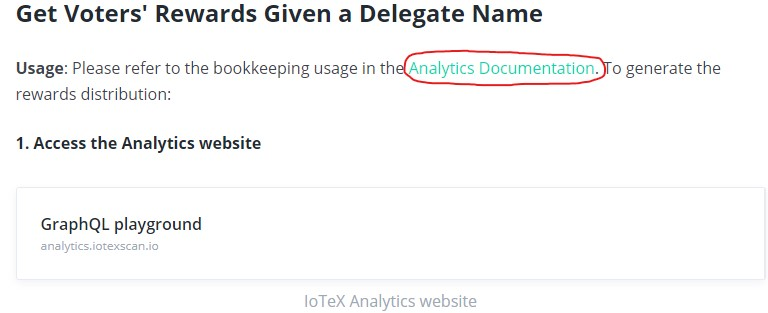
\includegraphics{images/analytics_documentation.jpg}

This is a really tiny typo, but pointing it out anyway; missing a
closing parenthesis here:

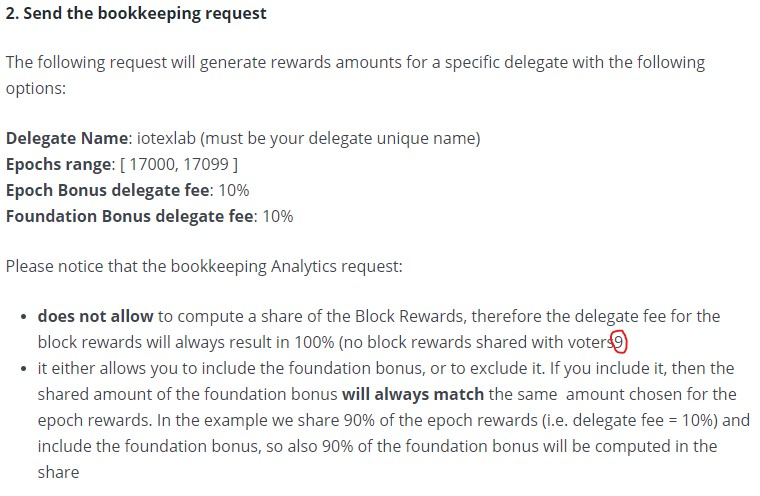
\includegraphics{images/missing_parentheses.jpg}

\hypertarget{basic-concepts}{%
\chapter{Basic Concepts}\label{basic-concepts}}

I really like the inclusion of this section. But I definitely think this
area of the documentation should be highlighted a lot more from the
start. Under \textbf{\emph{Software Tools -\textgreater{} Get Started}},
I think there should be some type of reference/links to the
\textbf{\emph{Basic Concepts}}. Nice graphics too, I like the one on the
\textbf{\emph{Blockchain Nodes}} section. I think fleshing out the
\textbf{\emph{Basic Concepts}} section as a whole would be valuable for
people just getting started.

\hypertarget{system-info}{%
\chapter{System Info}\label{system-info}}

For screenshots running Linux commands, here is some info about that
machine:

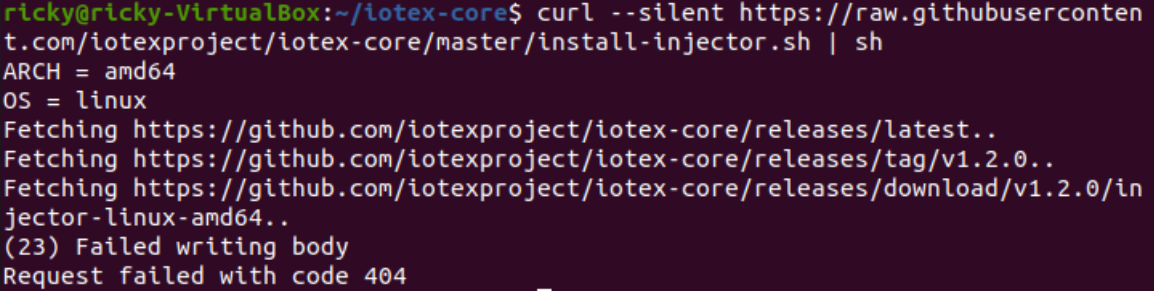
\includegraphics{images/linux_info.PNG}

\backmatter
\end{document}
